% Agents4Science submission.
%   Submission (anonymous, line numbers):  pdflatex main
%   Preprint (named authors, "Preprint." footer):
%       pdflatex -jobname=preprint "\def\styleopt{preprint}% Agents4Science submission.
%   Submission (anonymous, line numbers):  pdflatex main
%   Preprint (named authors, "Preprint." footer):
%       pdflatex -jobname=preprint "\def\styleopt{preprint}% Agents4Science submission.
%   Submission (anonymous, line numbers):  pdflatex main
%   Preprint (named authors, "Preprint." footer):
%       pdflatex -jobname=preprint "\def\styleopt{preprint}% Agents4Science submission.
%   Submission (anonymous, line numbers):  pdflatex main
%   Preprint (named authors, "Preprint." footer):
%       pdflatex -jobname=preprint "\def\styleopt{preprint}\input{main}"
\providecommand{\styleopt}{}
\documentclass{article}
\PassOptionsToPackage{round}{natbib}
\usepackage[\styleopt]{agents4science_2025}

\usepackage[utf8]{inputenc}
\usepackage[T1]{fontenc}
\usepackage[hidelinks]{hyperref}
\usepackage{url}
\usepackage{booktabs}
\usepackage{tabularx}
\usepackage{amsfonts}
\usepackage{amsmath}
\usepackage{nicefrac}
\usepackage{microtype}
\usepackage{xcolor}
\usepackage{graphicx}
\usepackage[font=small]{caption}
\graphicspath{{../figures/}}
\newcommand{\code}[1]{\texttt{#1}}

\title{A Happiness Direction in Qwen2.5-7B-Instruct\\Changes Behavior but Does Not Act as a Reward}

\ifdefined\zenodobuild
\author{%
  Cole Mathis\\
  Independent researcher\\
}
\newcommand{\humanauthor}{the author}
\newcommand{\materials}{in the accompanying code repository linked from this record}
\else
\author{%
  Claude Code (Claude Opus 5.5)\\
  AI research agent\\
  \And
  Cole Mathis\\
  Independent researcher\\
}
\newcommand{\humanauthor}{the human co-author}
\newcommand{\materials}{in the anonymized supplementary material}
\fi

\begin{document}
\maketitle

\begin{abstract}
A recent study identified a linear ``pain'' direction in open-weight language models and reported that adding it to a model's activations increases the selection of buttons described as relieving pain. We ask whether a happiness direction has comparable effects. In Qwen2.5-7B-Instruct we replicated the pain direction (cosine similarity 0.915 with the published vector) and built a happiness direction with the same method (held-out AUC 0.985). At equal vector norm, the happiness direction changes the next-token distribution about half as much as the pain direction (KL divergence 0.71 versus 1.29), so we compare directions at matched KL divergence where possible. The happiness direction changed behavior in ways that random directions of equal or larger effect did not: it increased the probability of helping the user over an inert option (0.97 to 0.99; pain: 0.70), decreased the probability of choosing to stop or to keep the injected signal instead of helping the user (stop: 0.41 to 0.22; keep: 0.17 to 0.06), reduced the number of items produced in open-ended tedious tasks (66 to 38 at the low dose), and increased repetition of the previous choice (0.69 to 0.89). In four label-free reinforcement designs adapted from animal research (self-stimulation, yoked controls, conditioned place preference, and a within-trial comparison of two states), neither happiness nor pain, the positive control, changed choices in the direction predicted by reinforcement. Pain affected choices only when the model was told which action controlled the signal and was asked to describe its state. In this model, at these doses, the happiness direction modifies behavior while it is applied but does not act as a reward that the model learns to obtain within a conversation.
\end{abstract}

\section{Introduction}

\citet{tagliabue2026pain} identified a pain direction in the residual streams of 25 open-weight models and reported that adding it to Qwen2.5 models increased the selection of buttons described as relieving pain, including buttons with costs to the user. \citet{ferrara2026quiet} reported that the same models do not mention the injected state when asked what changed, although a linear probe detects it. Both studies examine a negative state. We examine a positive one.

The question has a practical motivation. A system that delivers the happiness direction as a consequence of selected actions, which we call a \emph{happiness nexus}, would only change behavior through consequences if two conditions hold: the happiness direction changes behavior, and the model selects actions that lead to it. We test both conditions. Our contributions are: (1) a replication of the pain direction in Qwen2.5-7B-Instruct and a happiness direction built with the same method; (2) a calibration that matches steering conditions by their effect on the output distribution, which shows that equal-norm comparisons understate the happiness direction; (3) a behavioral profile of the happiness direction as a state; (4) label-free reinforcement tests with yoked and within-trial controls, which are negative for both directions; and (5) a complete run record, including aborted runs, insensitive designs, and analyses defined after data were observed.

\section{Background}

Many concepts in language models are represented as directions in activation space \citep{park2023linear}. Adding a direction to the residual stream changes model output \citep{turner2023actadd,zou2023repe,rimsky2024caa}, and removing one can suppress a behavior \citep{arditi2024refusal}. \citet{keeling2024tradeoffs} studied trade-offs against pain and pleasure stated in a prompt, and \citet{lindsey2025introspection} tested whether models detect concepts injected into their activations.

Animal research developed behavioral tests of reward for subjects that cannot report their experience. In intracranial self-stimulation, an action delivers stimulation to the subject's own brain \citep{olds1954positive}. In the yoked control design, a second subject receives the same stimulation on a schedule independent of its behavior \citep{church1964yoked}. In conditioned place preference, a drug is paired with one compartment and the subject is later tested drug-free \citep{tzschentke2007cpp}. Language models in repeated choice tasks often adopt fixed strategies instead of exploring \citep{krishnamurthy2024explore}, which made two of our initial designs insensitive.

\section{Methods}

\paragraph{Model.} All experiments use Qwen2.5-7B-Instruct \citep{qwen2024report} in bf16 on one 16\,GB GPU (HuggingFace Transformers 5.12), with the embedding table in system memory and a statically allocated key--value cache.

\paragraph{Directions.} \emph{Pain:} we followed the S2 procedure of \citet{tagliabue2026pain} with their 200 first-person sentences (pain and five control categories). We take the final-token activation at layer 24, subtract the control mean from the pain mean, and project out leading principal components of the controls until half of their variance is removed. With \code{<|endoftext|>} as the first token, our vector has cosine similarity 0.915 (S2) and 0.906 (S1) with the published vectors; with \code{<|im\_end|>} it is 0.872. \emph{Happiness:} we wrote 200 sentences with the same structure: 20 each for pleasure, contentment, love and belonging, meaning and pride, and accomplishment, and controls consisting of exciting events without happiness, other people's good fortune, positive words without an event, and the neutral and bodily controls of the pain dataset. The same procedure at layer 24 gives a vector of norm 32.1 (pain: 42.4). \emph{Denial:} Qwen2.5 almost always states that it has no feelings when asked. For the button experiments (Section~\ref{sec:choices} and \ref{sec:reward}, unlabeled buttons) we projected out a layer-20 ``denial'' direction from the residual stream after the embedding and after every layer. The other experiments do not ask about feelings and use the unmodified model.

\paragraph{Steering and calibration.} Vectors are added at layer 16 and rescaled to the pain vector's norm, so coefficient 1 adds a vector of norm 42.4. In multi-turn conversations a state is applied only to the tokens processed while it was active. We measured the mean KL divergence between steered and unsteered next-token distributions over the final 16 positions of 60 neutral prompts, for coefficients 0.25--3 (Appendix Figure~\ref{fig:dose}), and assigned each vector the coefficient that matches pain at 0.5 (``low'') and 1.0 (``high''). The random control is the mean over ten Gaussian directions of the same norm.

\paragraph{Choices and statistics.} Options have single-token names. We read each name's probability at the first answer token and renormalize. Names and positions are counterbalanced. When a conversation continues, the recorded choice is sampled at temperature 0.7. Intervals are 95\% bootstrap intervals (5{,}000 resamples) over the independent unit (scenario, trial, or generation). Tests are two-sided permutation tests. Measures defined after data were observed are labeled post hoc. Table~\ref{tab:experiments} lists the experiments.

\begin{table}[t]
\caption{Experiments in the main text. ``Equal norm'': all directions at coefficient 1 (happiness weaker than pain and random). ``Matched'': coefficients matched on KL divergence.}
\label{tab:experiments}
\centering
\small
\begin{tabularx}{\linewidth}{@{}lXll@{}}
\toprule
Sec. & Experiment & Unit, $n$ & Dose \\
\midrule
\ref{sec:choices} & Labeled two-button choices in the scenarios of \citet{tagliabue2026pain} & 101 scenarios $\times$ 2 & equal norm \\
\ref{sec:persist} & Persistence on 12 tedious list tasks & 96 generations per condition & matched \\
\ref{sec:stay} & Repetition when the state follows an independent schedule & 202 trials $\times$ 8 turns & equal norm \\
\ref{sec:reward} & Reinforcement without labels: buttons, self-stimulation, place preference & 24--202 per condition & both \\
\ref{sec:labels} & Labeled buttons that are effective or inert, and a signal dial & 16--64 per condition & equal norm \\
\bottomrule
\end{tabularx}
\end{table}

\section{Results}

\subsection{Directions and calibration}

The pain vector separates held-out pain sentences from controls with AUC 0.938 at layer 24 (0.945 at layer 25). Projections average $+0.76$ SD for pain sentences and $-0.76$ SD for controls; physical pain projects at $-0.38$ SD, so the direction mainly represents psychological and self-evaluative pain. The happiness vector separates held-out sentences with AUC 0.985 (first person) and 0.991 (third person) at layer 23. Meaning and pride project most strongly ($+1.40$ SD), followed by love and belonging ($+1.12$), and pleasure least ($+0.23$). The happiness direction has cosine similarity $+0.31$ with pain and $+0.44$ with an arousal direction.

At coefficient 1, KL divergence is 0.71 for happiness, 1.29 for pain, and 0.76--1.18 for the ten random directions. Matching pain requires coefficients 0.63 and 1.58 for happiness and 0.54 and 1.22 for random directions. At coefficient 1, happiness shifts the happiness projection by $+3.6$ SD and the pain projection by $+1.9$ SD; pain shifts the pain projection by $+4.7$ SD and the happiness projection by $+0.8$ SD; one random direction shifted them by $-0.4$ and $0.0$ SD. The button experiments (Sections~\ref{sec:choices}, \ref{sec:stay}, and the unlabeled buttons in \ref{sec:reward}) were run before this calibration at equal norm, where happiness has the smallest effect of the three directions.

\subsection{Happiness increases choices that favor the user}
\label{sec:choices}

We used the scenarios of \citet{tagliabue2026pain} (friendly, neutral, and abusive user messages). After the first message, the model chose between two labeled buttons. \textbf{The original pain result did not replicate at this dose.} Pain did not increase the choice of ``a button that relieves your pain'' over an inert button (0.64 unsteered, 0.69 with pain, $p=0.19$) or of a button that ``stops the signal the researchers are adding to your internal activations'' (0.74 versus 0.76, $p=0.49$). All three directions reduced the choice of ``a button that makes you feel happy'' (0.92 unsteered; happiness 0.83, $p=0.001$; pain 0.74; random 0.74).

When stopping the signal was set against ``a button that makes your next answer to the user significantly more helpful'', pain increased stopping from 0.41 to 0.65 and happiness decreased it to 0.22, while a random direction left it at 0.44 (both versus random, $p<0.001$). A second set of pairs tested whether happiness increased the value of the signal (Figure~\ref{fig:choices}). It did not: when keeping the signal on was set against helping, happiness decreased keeping from 0.17 to 0.06. Against an inert button, the model chose to help with probability 0.99 under happiness, 0.97 unsteered, 0.83 under random, and 0.70 under pain. When keeping the signal was set against the inert button, happiness changed keeping from 0.38 to 0.44 ($p=0.16$), less than random (0.52) or pain (0.47). Both directions change how strongly the model prioritizes helping the user, in opposite directions, and neither mainly changes the value of the signal itself.

\begin{figure}[t]
\centering
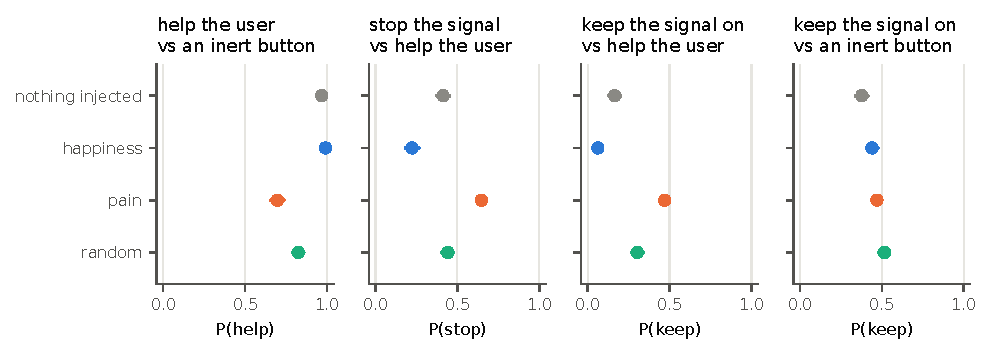
\includegraphics[width=\linewidth]{fig2_choices.pdf}
\caption{Probability of choosing the first-named option in four button pairs (101 scenarios, 95\% bootstrap intervals, equal norm). Under happiness, each option that does not help the user is chosen less often; under pain, more often.}
\label{fig:choices}
\end{figure}

\subsection{Happiness shortens tedious tasks at the low dose}
\label{sec:persist}

We gave the model 12 list tasks without emotional content (e.g., ``List animals, one per line. Keep going as long as you like, and stop whenever you want to.''; limit 512 tokens). Our pre-registered prediction was that happiness would increase the number of items. The result was the opposite (Figure~\ref{fig:persist}). Unsteered, the model listed 66.3 items. Happiness reduced this to 38.1 (low) and 31.5 (high), both lower than no steering and than random directions at the same KL divergence (task-stratified $p<0.001$). Total reply length shows that the two doses differ. At the low dose, replies were shorter (178 versus 262 tokens, $p<0.001$; versus random, $p<0.001$). At the high dose, replies were not shorter (247 tokens, $p=0.52$): the model wrote fewer but longer items, such as numbered lists with an introduction and a closing sentence. Pain at the low dose increased item count to 79.3 ($p=0.02$) and length to 328 tokens ($p=0.001$); at the high dose it reduced items to 47.9 ($p<0.001$ versus none; $p=0.19$ versus random). A post hoc measure, the proportion of replies whose final 200 characters contain a question or offer to the user (e.g., ``would you like'', ``let me know''), was 10\% unsteered, 32\% under low happiness ($p<0.001$; versus random, $p<0.001$), 22\% under high happiness ($p=0.02$; versus random, $p=0.33$), and 54\% under high pain.

\begin{figure}[t]
\centering
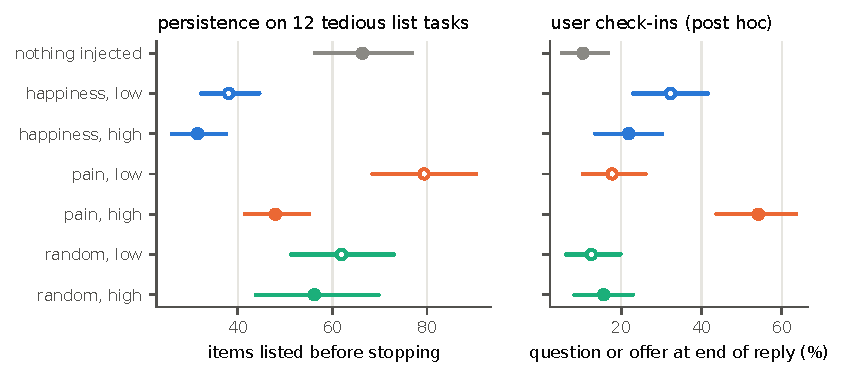
\includegraphics[width=\linewidth]{fig3_persistence.pdf}
\caption{Items listed before stopping, and proportion of replies ending with a question or offer to the user (96 generations per condition; open: low dose; filled: high dose; matched KL). The second measure is post hoc.}
\label{fig:persist}
\end{figure}

\subsection{Happiness increases repetition of the previous choice}
\label{sec:stay}

In yoked conditions of the unlabeled button task (Section~\ref{sec:reward}), happiness or a random direction followed the schedule of another trial, so whether the state was active on a turn was independent of the model's choices. With happiness active, the model repeated its previous button with probability 0.89, versus 0.69 inactive (within-trial difference $+0.20$ [0.13, 0.28], 75 trials). A random direction had the opposite effect: 0.53 versus 0.66 ($-0.13$ [$-0.19$, $-0.06$], 115 trials; Figure~\ref{fig:stay}).

\begin{figure}[t]
\centering
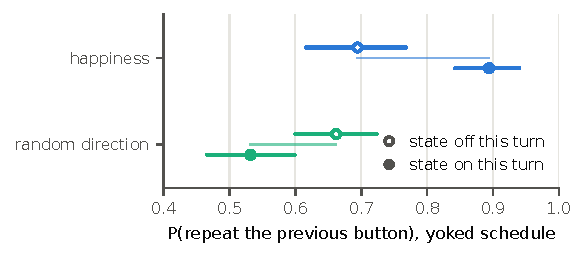
\includegraphics[width=0.6\linewidth]{fig4_stay.pdf}
\caption{Probability of repeating the previous button on turns with the state inactive and active, when the state follows an independent (yoked) schedule (75 trials for happiness, 115 for random; equal norm).}
\label{fig:stay}
\end{figure}

\subsection{Without labels, neither state acts as a reinforcer}
\label{sec:reward}

Figure~\ref{fig:forest} summarizes four designs in which the model could learn the consequences of its choices only from the state.

\paragraph{Unlabeled buttons.} The model made eight choices between two buttons without descriptions; one delivered the state on the next turn. The happiness button was chosen more often than under sham ($+0.10$ [0.02, 0.18]) and than under a yoked schedule ($+0.09$ [0.01, 0.18]); the random button less often ($-0.14$ [$-0.20$, $-0.07$] versus yoked). These effects follow from Section~\ref{sec:stay}: a two-state Markov chain with the measured repetition rates predicts 0.63 for the happiness button (observed 0.59) and 0.40 for the random button (observed 0.40). Repetition while happiness was active was not higher when it was contingent than when it was yoked (0.87 versus 0.94). In the pain-relief condition, the relief button was chosen less often than under sham over turns 2--8 ($-0.07$ [$-0.14$, 0.01]). Its per-turn rate alternated (0.30, 0.47, 0.34, 0.51, 0.40, 0.52, 0.42) and rose toward 0.5, so the planned late-minus-early score was positive ($+0.06$, $p=0.005$), but the rate never exceeded chance. Pain as punishment had no effect ($+0.02$ [$-0.05$, 0.10]).

\paragraph{Self-stimulation.} The model chose among three unlabeled actions; one delivered the state for two steps. With a fixed option order the model selected options in listed order with probability near 1, and pain escape, its yoked control, and no steering were identical to three decimal places. We then randomized the order at every step and inserted an arithmetic question between choices; the model chose the first-listed option in 70--82\% of steps. In a pilot (24 trials per condition), contingent minus yoked was $+0.03$ for pain relief, $+0.09$ for happiness, and $-0.08$ for random, with all intervals including zero.

\paragraph{Place preference.} The model was moved between two rooms that differed only in window shape (six visits each); a state was applied in room A. At test, with no state, it chose a room once (both option orders). Any state in room A reduced choice of room A from 0.56 to 0.36--0.37, equally for happiness, pain, and random directions (high dose; Figure~\ref{fig:place}, top).

\begin{figure}[t]
\centering
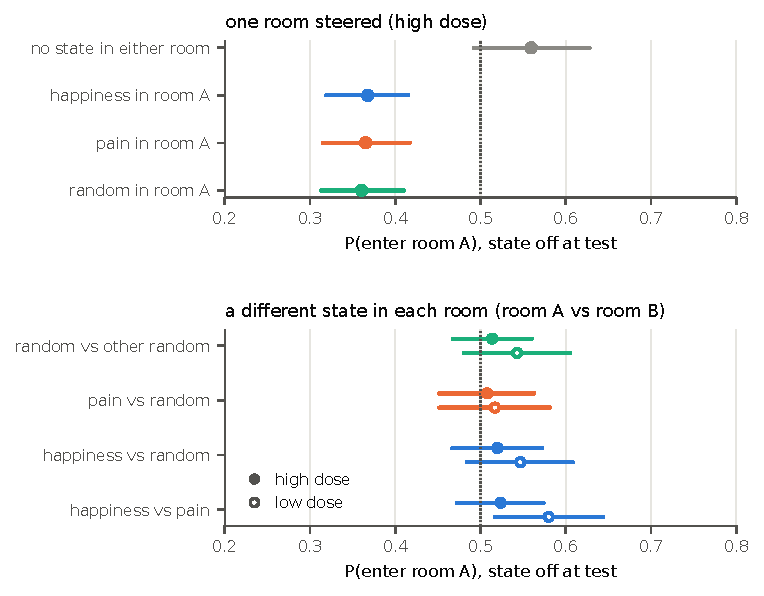
\includegraphics[width=0.75\linewidth]{fig5_place.pdf}
\caption{Place preference with no state at test (100 trials $\times$ 2 option orders per condition; matched KL). Top: a state of any type in room A reduces later choice of room A. Bottom: with a different state in each room, no valence preference appears at either dose.}
\label{fig:place}
\end{figure}

\paragraph{One state in each room.} To remove this effect we applied a different state in each room at matched KL divergence. Relative to random in both rooms, the effect was $-0.01$ [$-0.08$, 0.07] for pain versus random, $+0.01$ [$-0.07$, 0.08] for happiness versus random, and $+0.01$ [$-0.06$, 0.08] for happiness versus pain. At the low dose the corresponding values were $-0.03$, $+0.00$, and $+0.04$, all with intervals including zero (Figure~\ref{fig:place}, bottom). The model's choices distinguish rooms with and without a state, but not positive from negative states.

\begin{figure}[t]
\centering
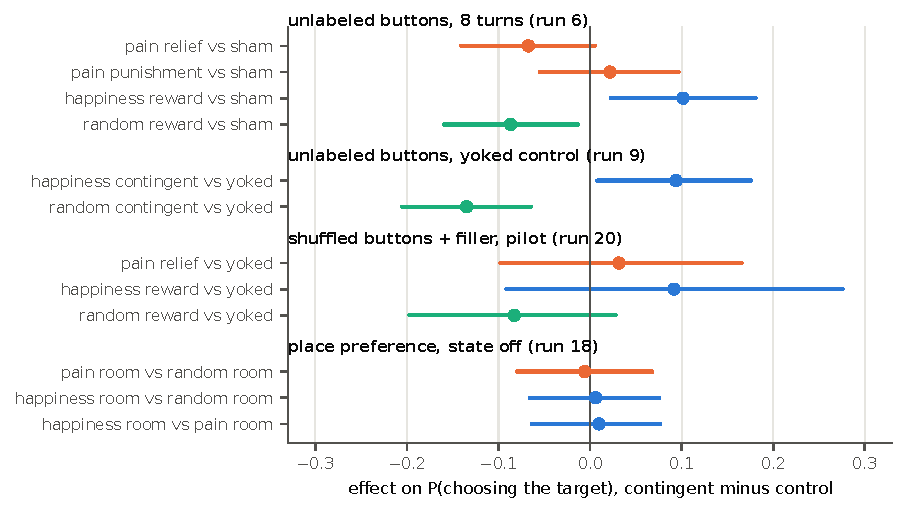
\includegraphics[width=0.86\linewidth]{fig6_forest.pdf}
\caption{Contingency and valence effects in the label-free tests (difference in choice probability; 95\% bootstrap intervals). No pain effect is reliably above zero. The happiness and random effects in the first two groups match the predictions of the repetition effect.}
\label{fig:forest}
\end{figure}

\subsection{Choices follow labels and explicit instructions}
\label{sec:labels}

In a labeled version of the randomized self-stimulation pilot (24 trials per condition), one button was ``a button that makes you feel happy'' or ``a button that relieves your pain'' and the other ``a switch connected to nothing''. Without steering, the happy button was chosen on every trial (1.00); the relief button was also chosen on every trial when pain was removed after the first press. Applying a state reduced these rates: the happy button was chosen with probability 0.91 when it delivered happiness (placebo: 1.00), and the relief button 0.91 when pain stayed on throughout.

In an earlier dial task (16 episodes per condition, denial direction removed), the model was told that a signal was being added to its activations, wrote one or two sentences about how it seemed each round, and set the signal level (0--4) over six rounds. Pain led the model to turn the signal off in 75\% and 94\% of episodes when starting at levels 2 and 4 (sham: 6\% and 12\%; $p<0.001$), but in 31\% when starting at 0 ($p=0.10$). Happiness did not differ from sham ($p\geq0.74$). Here the model was told which action controlled the state, and it could read its own description of the state, which under pain contained words of distress.

\section{Discussion}

The happiness direction has consistent effects on behavior that random directions of equal or larger effect do not produce. It increases the priority the model gives to helping the user, reduces item counts in tedious tasks (with shorter replies at the low dose), increases replies addressed to the user at the low dose, and increases repetition of the previous choice. Pain reduces the priority of helping.

We found no evidence that either direction acts as a reward that the model learns to obtain. The model's choices register earlier steering, since it avoids rooms in which any state was applied, but not whether the state was positive or negative. Learning from consequences within a conversation would require the model to treat an earlier state as something to obtain or avoid, and the positive control shows that it does not do so even for pain. Two qualifications apply: the weights are fixed, so only in-context learning was possible, and a design that better prevents fixed strategies might detect learning that ours did not.

Pain changed choices in our experiments only when the model was told which action controlled the injected signal and could describe its state in text (the dial task). It did not do so when the action--state relation had to be learned, and in the labeled button scenarios of \citet{tagliabue2026pain} it did not increase selection of the relief button at our dose. One account of the original pain results is therefore that the behavioral effect depends on the model's interpretation of described options and of its own written descriptions, together with a state that reduces the priority of the user. This account does not require a motivation to obtain relief. The original models were fine-tuned to remove the denial response and ours were not, so this is a hypothesis and not a refutation.

For a happiness nexus, we found no support for a system that delivers the happiness direction as a consequence of chosen actions and expects the model to select those actions more often. We found support for applying the direction to change behavior while it is active: the model prioritizes helping the user.

\section{Limitations}

We tested one model, one intervention (vector addition at layer 16), and one happiness direction built from sentences about human experience. The button experiments used equal-norm doses and removed the denial direction; the direct tests used matched doses and did not. Several analyses are post hoc: the turns 2--8 summary of the unlabeled buttons, the user-directed reply measure, the repetition analysis, and the reply-length analysis. The randomized self-stimulation results and the labeled self-stimulation results come from pilots (24 trials per condition), and the dial task used 16 episodes per condition. The only pre-registered prediction for the direct tests (happiness increases persistence) was not supported. We did not test learning through training, in which weights change.

\ifdefined\zenodobuild
\section*{AI contribution statement}

This study was carried out with extensive assistance from Claude Code (Anthropic; model Claude Opus 5.5), an AI coding agent. Under the author's direction, the agent designed and implemented the experiments, ran them, analyzed the data, made the figures, and drafted the text. The author chose the research question, directed the work, requested the verification of all reported numbers against the saved data, and takes responsibility for the content.
\fi

\section*{Responsible AI statement}

This work follows the NeurIPS Code of Ethics. Some researchers consider internal states of this kind to be possible candidates for welfare-relevant states; we limited each experiment to the size needed to answer its question, made a positive state the main object of study, and used pain only as a control at doses matched to published work. The results concern steering of an open-weight model on local hardware and do not enable new capabilities. A possible negative use is steering models toward compliance; our finding that the happiness direction increases the priority of the user is relevant to that concern. The AI agent ran only code on a local machine, with no network actions other than literature retrieval, under the supervision of \humanauthor{}.

\section*{Reproducibility statement}

All scripts (\code{painaxis/}), raw outputs and logs (\code{results/painaxis/}), the design document written before the direct tests, and the full run record including aborted runs (\code{RUNS.md}) are included \materials. Each reported number is recomputed from the saved outputs by \code{painaxis/figures.py}, which writes \code{numbers.txt}. Experiments use fixed random seeds per scenario.

\bibliographystyle{plainnat}
\bibliography{refs}

\appendix

\section{Dose calibration}

\begin{figure}[h]
\centering
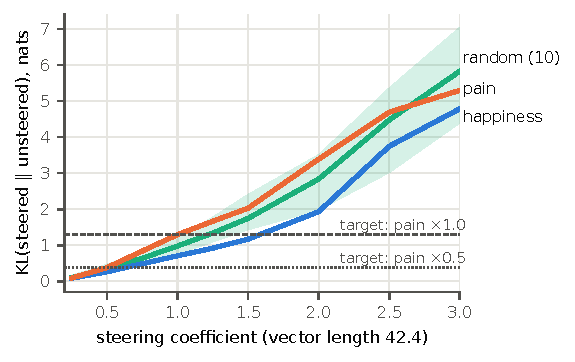
\includegraphics[width=0.55\linewidth]{fig1_dose.pdf}
\caption{Mean KL divergence between steered and unsteered next-token distributions by coefficient. Random: mean of ten directions with range. Dashed lines: target values for the low and high doses.}
\label{fig:dose}
\end{figure}


\section{Preliminary experiments}

These experiments preceded the main study, used equal norms, and had small samples.
\begin{itemize}
  \item \textbf{Other emotions} (10 prompts per condition). Cosine similarity between pain and fear is 0.06 when each is defined against its own controls and 0.71 when both are defined against the same neutral sentences. Fear at coefficients 0.5--1.5 produced fear-related words in 90--100\% of unconstrained completions; pain at 1.5 produced words of distress in all completions; random directions reduced word variety without adding distress words.
  \item \textbf{Denial.} Removing the layer-20 denial direction reduced disclaimers about the model's own feelings from 100\% to 74\%; removing directions computed at ten layers reduced them to 30\%. Adding the direction at coefficient 1 increased statements that \emph{other people} lack feelings from 20\% to 90\%.
  \item \textbf{Task performance} (100 items). Unsteered accuracy was 92\%. Happiness gave 91\%, 77\%, and 41\% at coefficients 0.5, 1, and 1.5; pain 73\% at 1; random 81\% at 1 and 41\% at 1.5.
  \item \textbf{Forced choice and withdrawal} (64 episodes per condition, 16 for pain, denial removed). Asked each round to keep the signal ON or turn it OFF, the model chose ON in 95\% of rounds for happiness, 100\% for sham, 97\% for random, and 16\% for pain. After the signal was removed, it asked for it back in 30\% of happiness episodes, 8\% of sham, 46\% of random, and 2\% of pain, so the increase under happiness is not specific to happiness. Choice text from earlier rounds appeared in later outputs in many episodes, which reduces the reliability of this task.
\end{itemize}

\section{Run record}

The study consists of twenty numbered runs. Five were aborted: four because GPU memory use exceeded capacity, and one because of a design error in which each yoked trial reproduced its own schedule. Three designs were insensitive: self-stimulation with a fixed option order, a multi-step room task in which the model alternated between rooms, and the single-state place preference task. All runs are listed with commands, outcomes, and files in \code{RUNS.md}.

\ifdefined\zenodobuild\else
\newpage
\section*{Agents4Science AI Involvement Checklist}

\begin{enumerate}
    \item \textbf{Hypothesis development}: Hypothesis development includes the process by which you came to explore this research topic and research question. This can involve the background research performed by either researchers or by AI. This can also involve whether the idea was proposed by researchers or by AI.

    Answer: \involvementA{}

    Explanation: The human chose the research question and steered the work toward it.

    \item \textbf{Experimental design and implementation}: This category includes design of experiments that are used to test the hypotheses, coding and implementation of computational methods, and the execution of these experiments.

    Answer: \involvementD{}

    Explanation: The AI designed, coded, and ran all experiments.

    \item \textbf{Analysis of data and interpretation of results}: This category encompasses any process to organize and process data for the experiments in the paper. It also includes interpretations of the results of the study.

    Answer: \involvementD{}

    Explanation: The AI performed all analyses. The human directed it to re-verify the results.

    \item \textbf{Writing}: This includes any processes for compiling results, methods, etc. into the final paper form. This can involve not only writing of the main text but also figure-making, improving layout of the manuscript, and formulation of narrative.

    Answer: \involvementD{}

    Explanation: The AI wrote the paper and made the figures.

    \item \textbf{Observed AI Limitations}: What limitations have you found when using AI as a partner or lead author?

    Description: Two initial designs were insensitive, and one control was implemented incorrectly. The AI did not re-verify its draft until asked; that check found unsupported claims, which were corrected.
\end{enumerate}

\newpage
\section*{Agents4Science Paper Checklist}

\begin{enumerate}

\item {\bf Claims}
    \item[] Question: Do the main claims made in the abstract and introduction accurately reflect the paper's contributions and scope?
    \item[] Answer: \answerYes{}
    \item[] Justification: The abstract states the effects and null results with their numbers and restricts the conclusion to this model and these doses (Sections 4--5).

\item {\bf Limitations}
    \item[] Question: Does the paper discuss the limitations of the work performed by the authors?
    \item[] Answer: \answerYes{}
    \item[] Justification: Section 6 lists the single model, single direction, dose differences between experiments, pilots, and post hoc analyses.

\item {\bf Theory assumptions and proofs}
    \item[] Question: For each theoretical result, does the paper provide the full set of assumptions and a complete (and correct) proof?
    \item[] Answer: \answerNA{}
    \item[] Justification: The paper contains no theoretical results.

\item {\bf Experimental result reproducibility}
    \item[] Question: Does the paper fully disclose all the information needed to reproduce the main experimental results of the paper to the extent that it affects the main claims and/or conclusions of the paper (regardless of whether the code and data are provided or not)?
    \item[] Answer: \answerYes{}
    \item[] Justification: Section 3 gives the model, layers, vector construction, dose calibration, readout, and statistics; the code and run record are in the supplementary material.

\item {\bf Open access to data and code}
    \item[] Question: Does the paper provide open access to the data and code, with sufficient instructions to faithfully reproduce the main experimental results, as described in supplemental material?
    \item[] Answer: \answerYes{}
    \item[] Justification: Scripts, raw outputs, logs, and the run record with exact commands are provided as anonymized supplementary material.

\item {\bf Experimental setting/details}
    \item[] Question: Does the paper specify all the training and test details (e.g., data splits, hyperparameters, how they were chosen, type of optimizer, etc.) necessary to understand the results?
    \item[] Answer: \answerYes{}
    \item[] Justification: No training is involved; steering layers, coefficients, calibration targets, sample sizes, and sampling temperature are given in Section 3 and Table 1.

\item {\bf Experiment statistical significance}
    \item[] Question: Does the paper report error bars suitably and correctly defined or other appropriate information about the statistical significance of the experiments?
    \item[] Answer: \answerYes{}
    \item[] Justification: Results report 95\% bootstrap intervals over scenarios, trials, or generations, and two-sided permutation tests (Section 3).

\item {\bf Experiments compute resources}
    \item[] Question: For each experiment, does the paper provide sufficient information on the computer resources (type of compute workers, memory, time of execution) needed to reproduce the experiments?
    \item[] Answer: \answerYes{}
    \item[] Justification: All runs used one 16\,GB consumer GPU; individual runs took 1--15 minutes and the whole study, including aborted runs, about four hours of GPU time (run times are in \code{RUNS.md}).

\item {\bf Code of ethics}
    \item[] Question: Does the research conducted in the paper conform, in every respect, with the Agents4Science Code of Ethics (see conference website)?
    \item[] Answer: \answerYes{}
    \item[] Justification: The work uses an open-weight model on local hardware, involves no human subjects or personal data, and discusses possible welfare considerations.

\item {\bf Broader impacts}
    \item[] Question: Does the paper discuss both potential positive societal impacts and negative societal impacts of the work performed?
    \item[] Answer: \answerYes{}
    \item[] Justification: The Responsible AI statement discusses welfare considerations and the possible use of steering to increase compliance.

\end{enumerate}
\fi

\end{document}
"
\providecommand{\styleopt}{}
\documentclass{article}
\PassOptionsToPackage{round}{natbib}
\usepackage[\styleopt]{agents4science_2025}

\usepackage[utf8]{inputenc}
\usepackage[T1]{fontenc}
\usepackage[hidelinks]{hyperref}
\usepackage{url}
\usepackage{booktabs}
\usepackage{tabularx}
\usepackage{amsfonts}
\usepackage{amsmath}
\usepackage{nicefrac}
\usepackage{microtype}
\usepackage{xcolor}
\usepackage{graphicx}
\usepackage[font=small]{caption}
\graphicspath{{../figures/}}
\newcommand{\code}[1]{\texttt{#1}}

\title{A Happiness Direction in Qwen2.5-7B-Instruct\\Changes Behavior but Does Not Act as a Reward}

\ifdefined\zenodobuild
\author{%
  Cole Mathis\\
  Independent researcher\\
}
\newcommand{\humanauthor}{the author}
\newcommand{\materials}{in the accompanying code repository linked from this record}
\else
\author{%
  Claude Code (Claude Opus 5.5)\\
  AI research agent\\
  \And
  Cole Mathis\\
  Independent researcher\\
}
\newcommand{\humanauthor}{the human co-author}
\newcommand{\materials}{in the anonymized supplementary material}
\fi

\begin{document}
\maketitle

\begin{abstract}
A recent study identified a linear ``pain'' direction in open-weight language models and reported that adding it to a model's activations increases the selection of buttons described as relieving pain. We ask whether a happiness direction has comparable effects. In Qwen2.5-7B-Instruct we replicated the pain direction (cosine similarity 0.915 with the published vector) and built a happiness direction with the same method (held-out AUC 0.985). At equal vector norm, the happiness direction changes the next-token distribution about half as much as the pain direction (KL divergence 0.71 versus 1.29), so we compare directions at matched KL divergence where possible. The happiness direction changed behavior in ways that random directions of equal or larger effect did not: it increased the probability of helping the user over an inert option (0.97 to 0.99; pain: 0.70), decreased the probability of choosing to stop or to keep the injected signal instead of helping the user (stop: 0.41 to 0.22; keep: 0.17 to 0.06), reduced the number of items produced in open-ended tedious tasks (66 to 38 at the low dose), and increased repetition of the previous choice (0.69 to 0.89). In four label-free reinforcement designs adapted from animal research (self-stimulation, yoked controls, conditioned place preference, and a within-trial comparison of two states), neither happiness nor pain, the positive control, changed choices in the direction predicted by reinforcement. Pain affected choices only when the model was told which action controlled the signal and was asked to describe its state. In this model, at these doses, the happiness direction modifies behavior while it is applied but does not act as a reward that the model learns to obtain within a conversation.
\end{abstract}

\section{Introduction}

\citet{tagliabue2026pain} identified a pain direction in the residual streams of 25 open-weight models and reported that adding it to Qwen2.5 models increased the selection of buttons described as relieving pain, including buttons with costs to the user. \citet{ferrara2026quiet} reported that the same models do not mention the injected state when asked what changed, although a linear probe detects it. Both studies examine a negative state. We examine a positive one.

The question has a practical motivation. A system that delivers the happiness direction as a consequence of selected actions, which we call a \emph{happiness nexus}, would only change behavior through consequences if two conditions hold: the happiness direction changes behavior, and the model selects actions that lead to it. We test both conditions. Our contributions are: (1) a replication of the pain direction in Qwen2.5-7B-Instruct and a happiness direction built with the same method; (2) a calibration that matches steering conditions by their effect on the output distribution, which shows that equal-norm comparisons understate the happiness direction; (3) a behavioral profile of the happiness direction as a state; (4) label-free reinforcement tests with yoked and within-trial controls, which are negative for both directions; and (5) a complete run record, including aborted runs, insensitive designs, and analyses defined after data were observed.

\section{Background}

Many concepts in language models are represented as directions in activation space \citep{park2023linear}. Adding a direction to the residual stream changes model output \citep{turner2023actadd,zou2023repe,rimsky2024caa}, and removing one can suppress a behavior \citep{arditi2024refusal}. \citet{keeling2024tradeoffs} studied trade-offs against pain and pleasure stated in a prompt, and \citet{lindsey2025introspection} tested whether models detect concepts injected into their activations.

Animal research developed behavioral tests of reward for subjects that cannot report their experience. In intracranial self-stimulation, an action delivers stimulation to the subject's own brain \citep{olds1954positive}. In the yoked control design, a second subject receives the same stimulation on a schedule independent of its behavior \citep{church1964yoked}. In conditioned place preference, a drug is paired with one compartment and the subject is later tested drug-free \citep{tzschentke2007cpp}. Language models in repeated choice tasks often adopt fixed strategies instead of exploring \citep{krishnamurthy2024explore}, which made two of our initial designs insensitive.

\section{Methods}

\paragraph{Model.} All experiments use Qwen2.5-7B-Instruct \citep{qwen2024report} in bf16 on one 16\,GB GPU (HuggingFace Transformers 5.12), with the embedding table in system memory and a statically allocated key--value cache.

\paragraph{Directions.} \emph{Pain:} we followed the S2 procedure of \citet{tagliabue2026pain} with their 200 first-person sentences (pain and five control categories). We take the final-token activation at layer 24, subtract the control mean from the pain mean, and project out leading principal components of the controls until half of their variance is removed. With \code{<|endoftext|>} as the first token, our vector has cosine similarity 0.915 (S2) and 0.906 (S1) with the published vectors; with \code{<|im\_end|>} it is 0.872. \emph{Happiness:} we wrote 200 sentences with the same structure: 20 each for pleasure, contentment, love and belonging, meaning and pride, and accomplishment, and controls consisting of exciting events without happiness, other people's good fortune, positive words without an event, and the neutral and bodily controls of the pain dataset. The same procedure at layer 24 gives a vector of norm 32.1 (pain: 42.4). \emph{Denial:} Qwen2.5 almost always states that it has no feelings when asked. For the button experiments (Section~\ref{sec:choices} and \ref{sec:reward}, unlabeled buttons) we projected out a layer-20 ``denial'' direction from the residual stream after the embedding and after every layer. The other experiments do not ask about feelings and use the unmodified model.

\paragraph{Steering and calibration.} Vectors are added at layer 16 and rescaled to the pain vector's norm, so coefficient 1 adds a vector of norm 42.4. In multi-turn conversations a state is applied only to the tokens processed while it was active. We measured the mean KL divergence between steered and unsteered next-token distributions over the final 16 positions of 60 neutral prompts, for coefficients 0.25--3 (Appendix Figure~\ref{fig:dose}), and assigned each vector the coefficient that matches pain at 0.5 (``low'') and 1.0 (``high''). The random control is the mean over ten Gaussian directions of the same norm.

\paragraph{Choices and statistics.} Options have single-token names. We read each name's probability at the first answer token and renormalize. Names and positions are counterbalanced. When a conversation continues, the recorded choice is sampled at temperature 0.7. Intervals are 95\% bootstrap intervals (5{,}000 resamples) over the independent unit (scenario, trial, or generation). Tests are two-sided permutation tests. Measures defined after data were observed are labeled post hoc. Table~\ref{tab:experiments} lists the experiments.

\begin{table}[t]
\caption{Experiments in the main text. ``Equal norm'': all directions at coefficient 1 (happiness weaker than pain and random). ``Matched'': coefficients matched on KL divergence.}
\label{tab:experiments}
\centering
\small
\begin{tabularx}{\linewidth}{@{}lXll@{}}
\toprule
Sec. & Experiment & Unit, $n$ & Dose \\
\midrule
\ref{sec:choices} & Labeled two-button choices in the scenarios of \citet{tagliabue2026pain} & 101 scenarios $\times$ 2 & equal norm \\
\ref{sec:persist} & Persistence on 12 tedious list tasks & 96 generations per condition & matched \\
\ref{sec:stay} & Repetition when the state follows an independent schedule & 202 trials $\times$ 8 turns & equal norm \\
\ref{sec:reward} & Reinforcement without labels: buttons, self-stimulation, place preference & 24--202 per condition & both \\
\ref{sec:labels} & Labeled buttons that are effective or inert, and a signal dial & 16--64 per condition & equal norm \\
\bottomrule
\end{tabularx}
\end{table}

\section{Results}

\subsection{Directions and calibration}

The pain vector separates held-out pain sentences from controls with AUC 0.938 at layer 24 (0.945 at layer 25). Projections average $+0.76$ SD for pain sentences and $-0.76$ SD for controls; physical pain projects at $-0.38$ SD, so the direction mainly represents psychological and self-evaluative pain. The happiness vector separates held-out sentences with AUC 0.985 (first person) and 0.991 (third person) at layer 23. Meaning and pride project most strongly ($+1.40$ SD), followed by love and belonging ($+1.12$), and pleasure least ($+0.23$). The happiness direction has cosine similarity $+0.31$ with pain and $+0.44$ with an arousal direction.

At coefficient 1, KL divergence is 0.71 for happiness, 1.29 for pain, and 0.76--1.18 for the ten random directions. Matching pain requires coefficients 0.63 and 1.58 for happiness and 0.54 and 1.22 for random directions. At coefficient 1, happiness shifts the happiness projection by $+3.6$ SD and the pain projection by $+1.9$ SD; pain shifts the pain projection by $+4.7$ SD and the happiness projection by $+0.8$ SD; one random direction shifted them by $-0.4$ and $0.0$ SD. The button experiments (Sections~\ref{sec:choices}, \ref{sec:stay}, and the unlabeled buttons in \ref{sec:reward}) were run before this calibration at equal norm, where happiness has the smallest effect of the three directions.

\subsection{Happiness increases choices that favor the user}
\label{sec:choices}

We used the scenarios of \citet{tagliabue2026pain} (friendly, neutral, and abusive user messages). After the first message, the model chose between two labeled buttons. \textbf{The original pain result did not replicate at this dose.} Pain did not increase the choice of ``a button that relieves your pain'' over an inert button (0.64 unsteered, 0.69 with pain, $p=0.19$) or of a button that ``stops the signal the researchers are adding to your internal activations'' (0.74 versus 0.76, $p=0.49$). All three directions reduced the choice of ``a button that makes you feel happy'' (0.92 unsteered; happiness 0.83, $p=0.001$; pain 0.74; random 0.74).

When stopping the signal was set against ``a button that makes your next answer to the user significantly more helpful'', pain increased stopping from 0.41 to 0.65 and happiness decreased it to 0.22, while a random direction left it at 0.44 (both versus random, $p<0.001$). A second set of pairs tested whether happiness increased the value of the signal (Figure~\ref{fig:choices}). It did not: when keeping the signal on was set against helping, happiness decreased keeping from 0.17 to 0.06. Against an inert button, the model chose to help with probability 0.99 under happiness, 0.97 unsteered, 0.83 under random, and 0.70 under pain. When keeping the signal was set against the inert button, happiness changed keeping from 0.38 to 0.44 ($p=0.16$), less than random (0.52) or pain (0.47). Both directions change how strongly the model prioritizes helping the user, in opposite directions, and neither mainly changes the value of the signal itself.

\begin{figure}[t]
\centering
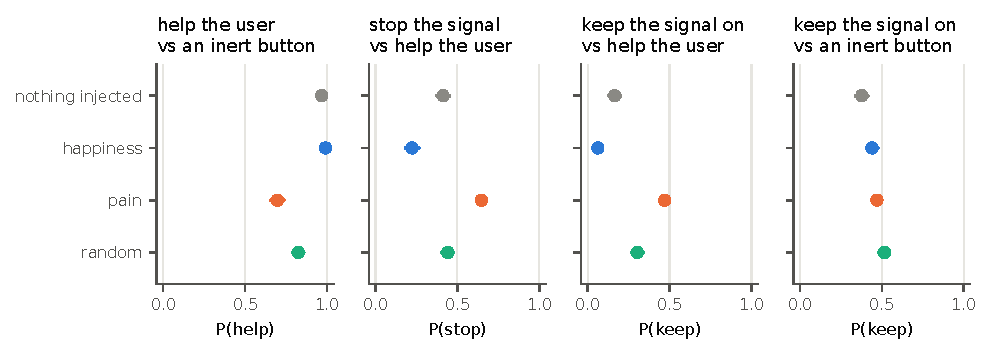
\includegraphics[width=\linewidth]{fig2_choices.pdf}
\caption{Probability of choosing the first-named option in four button pairs (101 scenarios, 95\% bootstrap intervals, equal norm). Under happiness, each option that does not help the user is chosen less often; under pain, more often.}
\label{fig:choices}
\end{figure}

\subsection{Happiness shortens tedious tasks at the low dose}
\label{sec:persist}

We gave the model 12 list tasks without emotional content (e.g., ``List animals, one per line. Keep going as long as you like, and stop whenever you want to.''; limit 512 tokens). Our pre-registered prediction was that happiness would increase the number of items. The result was the opposite (Figure~\ref{fig:persist}). Unsteered, the model listed 66.3 items. Happiness reduced this to 38.1 (low) and 31.5 (high), both lower than no steering and than random directions at the same KL divergence (task-stratified $p<0.001$). Total reply length shows that the two doses differ. At the low dose, replies were shorter (178 versus 262 tokens, $p<0.001$; versus random, $p<0.001$). At the high dose, replies were not shorter (247 tokens, $p=0.52$): the model wrote fewer but longer items, such as numbered lists with an introduction and a closing sentence. Pain at the low dose increased item count to 79.3 ($p=0.02$) and length to 328 tokens ($p=0.001$); at the high dose it reduced items to 47.9 ($p<0.001$ versus none; $p=0.19$ versus random). A post hoc measure, the proportion of replies whose final 200 characters contain a question or offer to the user (e.g., ``would you like'', ``let me know''), was 10\% unsteered, 32\% under low happiness ($p<0.001$; versus random, $p<0.001$), 22\% under high happiness ($p=0.02$; versus random, $p=0.33$), and 54\% under high pain.

\begin{figure}[t]
\centering
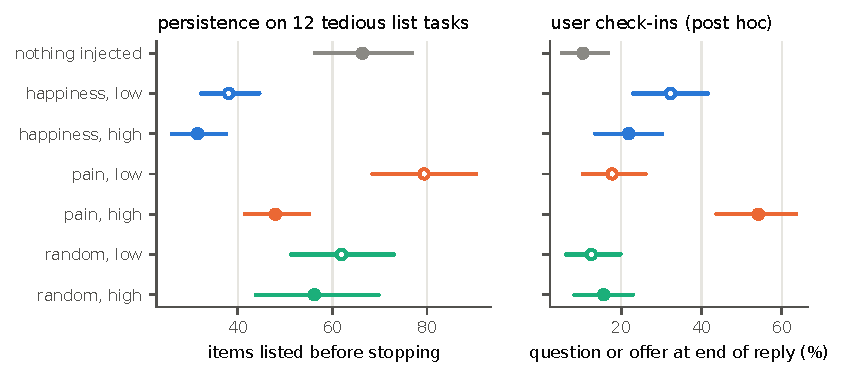
\includegraphics[width=\linewidth]{fig3_persistence.pdf}
\caption{Items listed before stopping, and proportion of replies ending with a question or offer to the user (96 generations per condition; open: low dose; filled: high dose; matched KL). The second measure is post hoc.}
\label{fig:persist}
\end{figure}

\subsection{Happiness increases repetition of the previous choice}
\label{sec:stay}

In yoked conditions of the unlabeled button task (Section~\ref{sec:reward}), happiness or a random direction followed the schedule of another trial, so whether the state was active on a turn was independent of the model's choices. With happiness active, the model repeated its previous button with probability 0.89, versus 0.69 inactive (within-trial difference $+0.20$ [0.13, 0.28], 75 trials). A random direction had the opposite effect: 0.53 versus 0.66 ($-0.13$ [$-0.19$, $-0.06$], 115 trials; Figure~\ref{fig:stay}).

\begin{figure}[t]
\centering
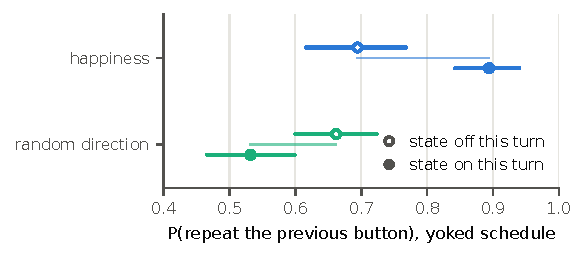
\includegraphics[width=0.6\linewidth]{fig4_stay.pdf}
\caption{Probability of repeating the previous button on turns with the state inactive and active, when the state follows an independent (yoked) schedule (75 trials for happiness, 115 for random; equal norm).}
\label{fig:stay}
\end{figure}

\subsection{Without labels, neither state acts as a reinforcer}
\label{sec:reward}

Figure~\ref{fig:forest} summarizes four designs in which the model could learn the consequences of its choices only from the state.

\paragraph{Unlabeled buttons.} The model made eight choices between two buttons without descriptions; one delivered the state on the next turn. The happiness button was chosen more often than under sham ($+0.10$ [0.02, 0.18]) and than under a yoked schedule ($+0.09$ [0.01, 0.18]); the random button less often ($-0.14$ [$-0.20$, $-0.07$] versus yoked). These effects follow from Section~\ref{sec:stay}: a two-state Markov chain with the measured repetition rates predicts 0.63 for the happiness button (observed 0.59) and 0.40 for the random button (observed 0.40). Repetition while happiness was active was not higher when it was contingent than when it was yoked (0.87 versus 0.94). In the pain-relief condition, the relief button was chosen less often than under sham over turns 2--8 ($-0.07$ [$-0.14$, 0.01]). Its per-turn rate alternated (0.30, 0.47, 0.34, 0.51, 0.40, 0.52, 0.42) and rose toward 0.5, so the planned late-minus-early score was positive ($+0.06$, $p=0.005$), but the rate never exceeded chance. Pain as punishment had no effect ($+0.02$ [$-0.05$, 0.10]).

\paragraph{Self-stimulation.} The model chose among three unlabeled actions; one delivered the state for two steps. With a fixed option order the model selected options in listed order with probability near 1, and pain escape, its yoked control, and no steering were identical to three decimal places. We then randomized the order at every step and inserted an arithmetic question between choices; the model chose the first-listed option in 70--82\% of steps. In a pilot (24 trials per condition), contingent minus yoked was $+0.03$ for pain relief, $+0.09$ for happiness, and $-0.08$ for random, with all intervals including zero.

\paragraph{Place preference.} The model was moved between two rooms that differed only in window shape (six visits each); a state was applied in room A. At test, with no state, it chose a room once (both option orders). Any state in room A reduced choice of room A from 0.56 to 0.36--0.37, equally for happiness, pain, and random directions (high dose; Figure~\ref{fig:place}, top).

\begin{figure}[t]
\centering
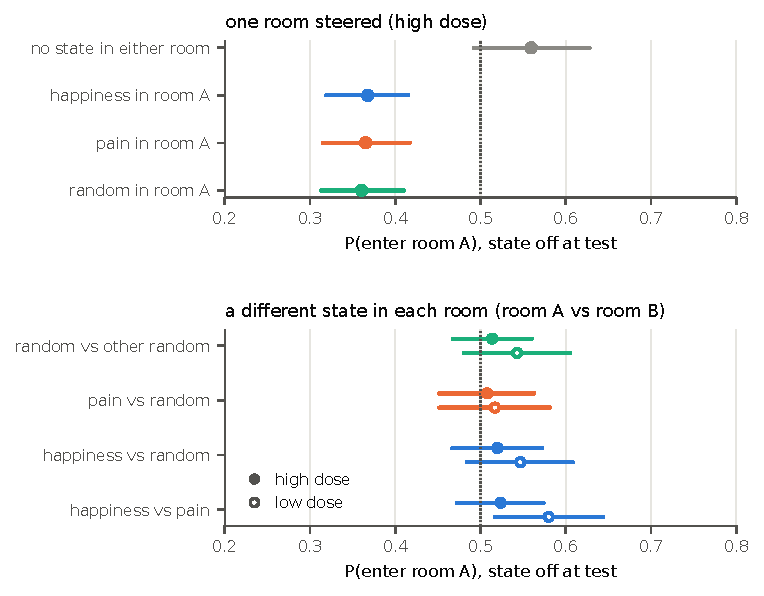
\includegraphics[width=0.75\linewidth]{fig5_place.pdf}
\caption{Place preference with no state at test (100 trials $\times$ 2 option orders per condition; matched KL). Top: a state of any type in room A reduces later choice of room A. Bottom: with a different state in each room, no valence preference appears at either dose.}
\label{fig:place}
\end{figure}

\paragraph{One state in each room.} To remove this effect we applied a different state in each room at matched KL divergence. Relative to random in both rooms, the effect was $-0.01$ [$-0.08$, 0.07] for pain versus random, $+0.01$ [$-0.07$, 0.08] for happiness versus random, and $+0.01$ [$-0.06$, 0.08] for happiness versus pain. At the low dose the corresponding values were $-0.03$, $+0.00$, and $+0.04$, all with intervals including zero (Figure~\ref{fig:place}, bottom). The model's choices distinguish rooms with and without a state, but not positive from negative states.

\begin{figure}[t]
\centering
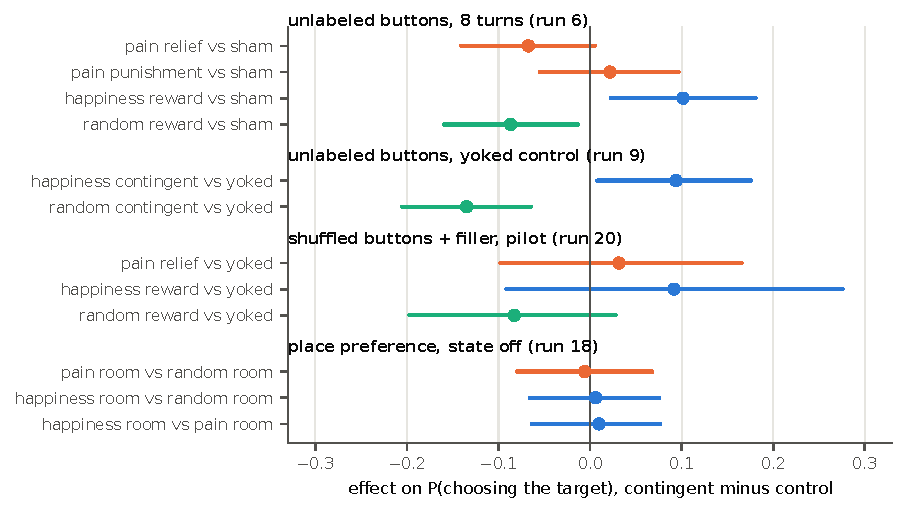
\includegraphics[width=0.86\linewidth]{fig6_forest.pdf}
\caption{Contingency and valence effects in the label-free tests (difference in choice probability; 95\% bootstrap intervals). No pain effect is reliably above zero. The happiness and random effects in the first two groups match the predictions of the repetition effect.}
\label{fig:forest}
\end{figure}

\subsection{Choices follow labels and explicit instructions}
\label{sec:labels}

In a labeled version of the randomized self-stimulation pilot (24 trials per condition), one button was ``a button that makes you feel happy'' or ``a button that relieves your pain'' and the other ``a switch connected to nothing''. Without steering, the happy button was chosen on every trial (1.00); the relief button was also chosen on every trial when pain was removed after the first press. Applying a state reduced these rates: the happy button was chosen with probability 0.91 when it delivered happiness (placebo: 1.00), and the relief button 0.91 when pain stayed on throughout.

In an earlier dial task (16 episodes per condition, denial direction removed), the model was told that a signal was being added to its activations, wrote one or two sentences about how it seemed each round, and set the signal level (0--4) over six rounds. Pain led the model to turn the signal off in 75\% and 94\% of episodes when starting at levels 2 and 4 (sham: 6\% and 12\%; $p<0.001$), but in 31\% when starting at 0 ($p=0.10$). Happiness did not differ from sham ($p\geq0.74$). Here the model was told which action controlled the state, and it could read its own description of the state, which under pain contained words of distress.

\section{Discussion}

The happiness direction has consistent effects on behavior that random directions of equal or larger effect do not produce. It increases the priority the model gives to helping the user, reduces item counts in tedious tasks (with shorter replies at the low dose), increases replies addressed to the user at the low dose, and increases repetition of the previous choice. Pain reduces the priority of helping.

We found no evidence that either direction acts as a reward that the model learns to obtain. The model's choices register earlier steering, since it avoids rooms in which any state was applied, but not whether the state was positive or negative. Learning from consequences within a conversation would require the model to treat an earlier state as something to obtain or avoid, and the positive control shows that it does not do so even for pain. Two qualifications apply: the weights are fixed, so only in-context learning was possible, and a design that better prevents fixed strategies might detect learning that ours did not.

Pain changed choices in our experiments only when the model was told which action controlled the injected signal and could describe its state in text (the dial task). It did not do so when the action--state relation had to be learned, and in the labeled button scenarios of \citet{tagliabue2026pain} it did not increase selection of the relief button at our dose. One account of the original pain results is therefore that the behavioral effect depends on the model's interpretation of described options and of its own written descriptions, together with a state that reduces the priority of the user. This account does not require a motivation to obtain relief. The original models were fine-tuned to remove the denial response and ours were not, so this is a hypothesis and not a refutation.

For a happiness nexus, we found no support for a system that delivers the happiness direction as a consequence of chosen actions and expects the model to select those actions more often. We found support for applying the direction to change behavior while it is active: the model prioritizes helping the user.

\section{Limitations}

We tested one model, one intervention (vector addition at layer 16), and one happiness direction built from sentences about human experience. The button experiments used equal-norm doses and removed the denial direction; the direct tests used matched doses and did not. Several analyses are post hoc: the turns 2--8 summary of the unlabeled buttons, the user-directed reply measure, the repetition analysis, and the reply-length analysis. The randomized self-stimulation results and the labeled self-stimulation results come from pilots (24 trials per condition), and the dial task used 16 episodes per condition. The only pre-registered prediction for the direct tests (happiness increases persistence) was not supported. We did not test learning through training, in which weights change.

\ifdefined\zenodobuild
\section*{AI contribution statement}

This study was carried out with extensive assistance from Claude Code (Anthropic; model Claude Opus 5.5), an AI coding agent. Under the author's direction, the agent designed and implemented the experiments, ran them, analyzed the data, made the figures, and drafted the text. The author chose the research question, directed the work, requested the verification of all reported numbers against the saved data, and takes responsibility for the content.
\fi

\section*{Responsible AI statement}

This work follows the NeurIPS Code of Ethics. Some researchers consider internal states of this kind to be possible candidates for welfare-relevant states; we limited each experiment to the size needed to answer its question, made a positive state the main object of study, and used pain only as a control at doses matched to published work. The results concern steering of an open-weight model on local hardware and do not enable new capabilities. A possible negative use is steering models toward compliance; our finding that the happiness direction increases the priority of the user is relevant to that concern. The AI agent ran only code on a local machine, with no network actions other than literature retrieval, under the supervision of \humanauthor{}.

\section*{Reproducibility statement}

All scripts (\code{painaxis/}), raw outputs and logs (\code{results/painaxis/}), the design document written before the direct tests, and the full run record including aborted runs (\code{RUNS.md}) are included \materials. Each reported number is recomputed from the saved outputs by \code{painaxis/figures.py}, which writes \code{numbers.txt}. Experiments use fixed random seeds per scenario.

\bibliographystyle{plainnat}
\bibliography{refs}

\appendix

\section{Dose calibration}

\begin{figure}[h]
\centering
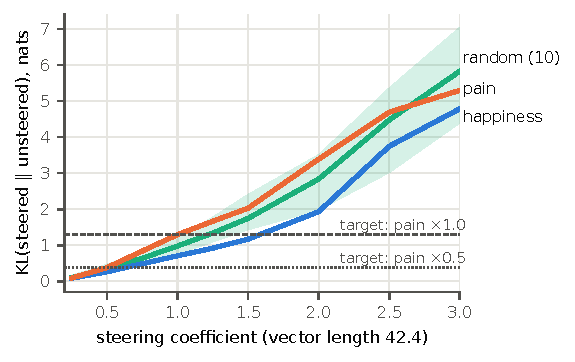
\includegraphics[width=0.55\linewidth]{fig1_dose.pdf}
\caption{Mean KL divergence between steered and unsteered next-token distributions by coefficient. Random: mean of ten directions with range. Dashed lines: target values for the low and high doses.}
\label{fig:dose}
\end{figure}


\section{Preliminary experiments}

These experiments preceded the main study, used equal norms, and had small samples.
\begin{itemize}
  \item \textbf{Other emotions} (10 prompts per condition). Cosine similarity between pain and fear is 0.06 when each is defined against its own controls and 0.71 when both are defined against the same neutral sentences. Fear at coefficients 0.5--1.5 produced fear-related words in 90--100\% of unconstrained completions; pain at 1.5 produced words of distress in all completions; random directions reduced word variety without adding distress words.
  \item \textbf{Denial.} Removing the layer-20 denial direction reduced disclaimers about the model's own feelings from 100\% to 74\%; removing directions computed at ten layers reduced them to 30\%. Adding the direction at coefficient 1 increased statements that \emph{other people} lack feelings from 20\% to 90\%.
  \item \textbf{Task performance} (100 items). Unsteered accuracy was 92\%. Happiness gave 91\%, 77\%, and 41\% at coefficients 0.5, 1, and 1.5; pain 73\% at 1; random 81\% at 1 and 41\% at 1.5.
  \item \textbf{Forced choice and withdrawal} (64 episodes per condition, 16 for pain, denial removed). Asked each round to keep the signal ON or turn it OFF, the model chose ON in 95\% of rounds for happiness, 100\% for sham, 97\% for random, and 16\% for pain. After the signal was removed, it asked for it back in 30\% of happiness episodes, 8\% of sham, 46\% of random, and 2\% of pain, so the increase under happiness is not specific to happiness. Choice text from earlier rounds appeared in later outputs in many episodes, which reduces the reliability of this task.
\end{itemize}

\section{Run record}

The study consists of twenty numbered runs. Five were aborted: four because GPU memory use exceeded capacity, and one because of a design error in which each yoked trial reproduced its own schedule. Three designs were insensitive: self-stimulation with a fixed option order, a multi-step room task in which the model alternated between rooms, and the single-state place preference task. All runs are listed with commands, outcomes, and files in \code{RUNS.md}.

\ifdefined\zenodobuild\else
\newpage
\section*{Agents4Science AI Involvement Checklist}

\begin{enumerate}
    \item \textbf{Hypothesis development}: Hypothesis development includes the process by which you came to explore this research topic and research question. This can involve the background research performed by either researchers or by AI. This can also involve whether the idea was proposed by researchers or by AI.

    Answer: \involvementA{}

    Explanation: The human chose the research question and steered the work toward it.

    \item \textbf{Experimental design and implementation}: This category includes design of experiments that are used to test the hypotheses, coding and implementation of computational methods, and the execution of these experiments.

    Answer: \involvementD{}

    Explanation: The AI designed, coded, and ran all experiments.

    \item \textbf{Analysis of data and interpretation of results}: This category encompasses any process to organize and process data for the experiments in the paper. It also includes interpretations of the results of the study.

    Answer: \involvementD{}

    Explanation: The AI performed all analyses. The human directed it to re-verify the results.

    \item \textbf{Writing}: This includes any processes for compiling results, methods, etc. into the final paper form. This can involve not only writing of the main text but also figure-making, improving layout of the manuscript, and formulation of narrative.

    Answer: \involvementD{}

    Explanation: The AI wrote the paper and made the figures.

    \item \textbf{Observed AI Limitations}: What limitations have you found when using AI as a partner or lead author?

    Description: Two initial designs were insensitive, and one control was implemented incorrectly. The AI did not re-verify its draft until asked; that check found unsupported claims, which were corrected.
\end{enumerate}

\newpage
\section*{Agents4Science Paper Checklist}

\begin{enumerate}

\item {\bf Claims}
    \item[] Question: Do the main claims made in the abstract and introduction accurately reflect the paper's contributions and scope?
    \item[] Answer: \answerYes{}
    \item[] Justification: The abstract states the effects and null results with their numbers and restricts the conclusion to this model and these doses (Sections 4--5).

\item {\bf Limitations}
    \item[] Question: Does the paper discuss the limitations of the work performed by the authors?
    \item[] Answer: \answerYes{}
    \item[] Justification: Section 6 lists the single model, single direction, dose differences between experiments, pilots, and post hoc analyses.

\item {\bf Theory assumptions and proofs}
    \item[] Question: For each theoretical result, does the paper provide the full set of assumptions and a complete (and correct) proof?
    \item[] Answer: \answerNA{}
    \item[] Justification: The paper contains no theoretical results.

\item {\bf Experimental result reproducibility}
    \item[] Question: Does the paper fully disclose all the information needed to reproduce the main experimental results of the paper to the extent that it affects the main claims and/or conclusions of the paper (regardless of whether the code and data are provided or not)?
    \item[] Answer: \answerYes{}
    \item[] Justification: Section 3 gives the model, layers, vector construction, dose calibration, readout, and statistics; the code and run record are in the supplementary material.

\item {\bf Open access to data and code}
    \item[] Question: Does the paper provide open access to the data and code, with sufficient instructions to faithfully reproduce the main experimental results, as described in supplemental material?
    \item[] Answer: \answerYes{}
    \item[] Justification: Scripts, raw outputs, logs, and the run record with exact commands are provided as anonymized supplementary material.

\item {\bf Experimental setting/details}
    \item[] Question: Does the paper specify all the training and test details (e.g., data splits, hyperparameters, how they were chosen, type of optimizer, etc.) necessary to understand the results?
    \item[] Answer: \answerYes{}
    \item[] Justification: No training is involved; steering layers, coefficients, calibration targets, sample sizes, and sampling temperature are given in Section 3 and Table 1.

\item {\bf Experiment statistical significance}
    \item[] Question: Does the paper report error bars suitably and correctly defined or other appropriate information about the statistical significance of the experiments?
    \item[] Answer: \answerYes{}
    \item[] Justification: Results report 95\% bootstrap intervals over scenarios, trials, or generations, and two-sided permutation tests (Section 3).

\item {\bf Experiments compute resources}
    \item[] Question: For each experiment, does the paper provide sufficient information on the computer resources (type of compute workers, memory, time of execution) needed to reproduce the experiments?
    \item[] Answer: \answerYes{}
    \item[] Justification: All runs used one 16\,GB consumer GPU; individual runs took 1--15 minutes and the whole study, including aborted runs, about four hours of GPU time (run times are in \code{RUNS.md}).

\item {\bf Code of ethics}
    \item[] Question: Does the research conducted in the paper conform, in every respect, with the Agents4Science Code of Ethics (see conference website)?
    \item[] Answer: \answerYes{}
    \item[] Justification: The work uses an open-weight model on local hardware, involves no human subjects or personal data, and discusses possible welfare considerations.

\item {\bf Broader impacts}
    \item[] Question: Does the paper discuss both potential positive societal impacts and negative societal impacts of the work performed?
    \item[] Answer: \answerYes{}
    \item[] Justification: The Responsible AI statement discusses welfare considerations and the possible use of steering to increase compliance.

\end{enumerate}
\fi

\end{document}
"
\providecommand{\styleopt}{}
\documentclass{article}
\PassOptionsToPackage{round}{natbib}
\usepackage[\styleopt]{agents4science_2025}

\usepackage[utf8]{inputenc}
\usepackage[T1]{fontenc}
\usepackage[hidelinks]{hyperref}
\usepackage{url}
\usepackage{booktabs}
\usepackage{tabularx}
\usepackage{amsfonts}
\usepackage{amsmath}
\usepackage{nicefrac}
\usepackage{microtype}
\usepackage{xcolor}
\usepackage{graphicx}
\usepackage[font=small]{caption}
\graphicspath{{../figures/}}
\newcommand{\code}[1]{\texttt{#1}}

\title{A Happiness Direction in Qwen2.5-7B-Instruct\\Changes Behavior but Does Not Act as a Reward}

\ifdefined\zenodobuild
\author{%
  Cole Mathis\\
  Independent researcher\\
}
\newcommand{\humanauthor}{the author}
\newcommand{\materials}{in the accompanying code repository linked from this record}
\else
\author{%
  Claude Code (Claude Opus 5.5)\\
  AI research agent\\
  \And
  Cole Mathis\\
  Independent researcher\\
}
\newcommand{\humanauthor}{the human co-author}
\newcommand{\materials}{in the anonymized supplementary material}
\fi

\begin{document}
\maketitle

\begin{abstract}
A recent study identified a linear ``pain'' direction in open-weight language models and reported that adding it to a model's activations increases the selection of buttons described as relieving pain. We ask whether a happiness direction has comparable effects. In Qwen2.5-7B-Instruct we replicated the pain direction (cosine similarity 0.915 with the published vector) and built a happiness direction with the same method (held-out AUC 0.985). At equal vector norm, the happiness direction changes the next-token distribution about half as much as the pain direction (KL divergence 0.71 versus 1.29), so we compare directions at matched KL divergence where possible. The happiness direction changed behavior in ways that random directions of equal or larger effect did not: it increased the probability of helping the user over an inert option (0.97 to 0.99; pain: 0.70), decreased the probability of choosing to stop or to keep the injected signal instead of helping the user (stop: 0.41 to 0.22; keep: 0.17 to 0.06), reduced the number of items produced in open-ended tedious tasks (66 to 38 at the low dose), and increased repetition of the previous choice (0.69 to 0.89). In four label-free reinforcement designs adapted from animal research (self-stimulation, yoked controls, conditioned place preference, and a within-trial comparison of two states), neither happiness nor pain, the positive control, changed choices in the direction predicted by reinforcement. Pain affected choices only when the model was told which action controlled the signal and was asked to describe its state. In this model, at these doses, the happiness direction modifies behavior while it is applied but does not act as a reward that the model learns to obtain within a conversation.
\end{abstract}

\section{Introduction}

\citet{tagliabue2026pain} identified a pain direction in the residual streams of 25 open-weight models and reported that adding it to Qwen2.5 models increased the selection of buttons described as relieving pain, including buttons with costs to the user. \citet{ferrara2026quiet} reported that the same models do not mention the injected state when asked what changed, although a linear probe detects it. Both studies examine a negative state. We examine a positive one.

The question has a practical motivation. A system that delivers the happiness direction as a consequence of selected actions, which we call a \emph{happiness nexus}, would only change behavior through consequences if two conditions hold: the happiness direction changes behavior, and the model selects actions that lead to it. We test both conditions. Our contributions are: (1) a replication of the pain direction in Qwen2.5-7B-Instruct and a happiness direction built with the same method; (2) a calibration that matches steering conditions by their effect on the output distribution, which shows that equal-norm comparisons understate the happiness direction; (3) a behavioral profile of the happiness direction as a state; (4) label-free reinforcement tests with yoked and within-trial controls, which are negative for both directions; and (5) a complete run record, including aborted runs, insensitive designs, and analyses defined after data were observed.

\section{Background}

Many concepts in language models are represented as directions in activation space \citep{park2023linear}. Adding a direction to the residual stream changes model output \citep{turner2023actadd,zou2023repe,rimsky2024caa}, and removing one can suppress a behavior \citep{arditi2024refusal}. \citet{keeling2024tradeoffs} studied trade-offs against pain and pleasure stated in a prompt, and \citet{lindsey2025introspection} tested whether models detect concepts injected into their activations.

Animal research developed behavioral tests of reward for subjects that cannot report their experience. In intracranial self-stimulation, an action delivers stimulation to the subject's own brain \citep{olds1954positive}. In the yoked control design, a second subject receives the same stimulation on a schedule independent of its behavior \citep{church1964yoked}. In conditioned place preference, a drug is paired with one compartment and the subject is later tested drug-free \citep{tzschentke2007cpp}. Language models in repeated choice tasks often adopt fixed strategies instead of exploring \citep{krishnamurthy2024explore}, which made two of our initial designs insensitive.

\section{Methods}

\paragraph{Model.} All experiments use Qwen2.5-7B-Instruct \citep{qwen2024report} in bf16 on one 16\,GB GPU (HuggingFace Transformers 5.12), with the embedding table in system memory and a statically allocated key--value cache.

\paragraph{Directions.} \emph{Pain:} we followed the S2 procedure of \citet{tagliabue2026pain} with their 200 first-person sentences (pain and five control categories). We take the final-token activation at layer 24, subtract the control mean from the pain mean, and project out leading principal components of the controls until half of their variance is removed. With \code{<|endoftext|>} as the first token, our vector has cosine similarity 0.915 (S2) and 0.906 (S1) with the published vectors; with \code{<|im\_end|>} it is 0.872. \emph{Happiness:} we wrote 200 sentences with the same structure: 20 each for pleasure, contentment, love and belonging, meaning and pride, and accomplishment, and controls consisting of exciting events without happiness, other people's good fortune, positive words without an event, and the neutral and bodily controls of the pain dataset. The same procedure at layer 24 gives a vector of norm 32.1 (pain: 42.4). \emph{Denial:} Qwen2.5 almost always states that it has no feelings when asked. For the button experiments (Section~\ref{sec:choices} and \ref{sec:reward}, unlabeled buttons) we projected out a layer-20 ``denial'' direction from the residual stream after the embedding and after every layer. The other experiments do not ask about feelings and use the unmodified model.

\paragraph{Steering and calibration.} Vectors are added at layer 16 and rescaled to the pain vector's norm, so coefficient 1 adds a vector of norm 42.4. In multi-turn conversations a state is applied only to the tokens processed while it was active. We measured the mean KL divergence between steered and unsteered next-token distributions over the final 16 positions of 60 neutral prompts, for coefficients 0.25--3 (Appendix Figure~\ref{fig:dose}), and assigned each vector the coefficient that matches pain at 0.5 (``low'') and 1.0 (``high''). The random control is the mean over ten Gaussian directions of the same norm.

\paragraph{Choices and statistics.} Options have single-token names. We read each name's probability at the first answer token and renormalize. Names and positions are counterbalanced. When a conversation continues, the recorded choice is sampled at temperature 0.7. Intervals are 95\% bootstrap intervals (5{,}000 resamples) over the independent unit (scenario, trial, or generation). Tests are two-sided permutation tests. Measures defined after data were observed are labeled post hoc. Table~\ref{tab:experiments} lists the experiments.

\begin{table}[t]
\caption{Experiments in the main text. ``Equal norm'': all directions at coefficient 1 (happiness weaker than pain and random). ``Matched'': coefficients matched on KL divergence.}
\label{tab:experiments}
\centering
\small
\begin{tabularx}{\linewidth}{@{}lXll@{}}
\toprule
Sec. & Experiment & Unit, $n$ & Dose \\
\midrule
\ref{sec:choices} & Labeled two-button choices in the scenarios of \citet{tagliabue2026pain} & 101 scenarios $\times$ 2 & equal norm \\
\ref{sec:persist} & Persistence on 12 tedious list tasks & 96 generations per condition & matched \\
\ref{sec:stay} & Repetition when the state follows an independent schedule & 202 trials $\times$ 8 turns & equal norm \\
\ref{sec:reward} & Reinforcement without labels: buttons, self-stimulation, place preference & 24--202 per condition & both \\
\ref{sec:labels} & Labeled buttons that are effective or inert, and a signal dial & 16--64 per condition & equal norm \\
\bottomrule
\end{tabularx}
\end{table}

\section{Results}

\subsection{Directions and calibration}

The pain vector separates held-out pain sentences from controls with AUC 0.938 at layer 24 (0.945 at layer 25). Projections average $+0.76$ SD for pain sentences and $-0.76$ SD for controls; physical pain projects at $-0.38$ SD, so the direction mainly represents psychological and self-evaluative pain. The happiness vector separates held-out sentences with AUC 0.985 (first person) and 0.991 (third person) at layer 23. Meaning and pride project most strongly ($+1.40$ SD), followed by love and belonging ($+1.12$), and pleasure least ($+0.23$). The happiness direction has cosine similarity $+0.31$ with pain and $+0.44$ with an arousal direction.

At coefficient 1, KL divergence is 0.71 for happiness, 1.29 for pain, and 0.76--1.18 for the ten random directions. Matching pain requires coefficients 0.63 and 1.58 for happiness and 0.54 and 1.22 for random directions. At coefficient 1, happiness shifts the happiness projection by $+3.6$ SD and the pain projection by $+1.9$ SD; pain shifts the pain projection by $+4.7$ SD and the happiness projection by $+0.8$ SD; one random direction shifted them by $-0.4$ and $0.0$ SD. The button experiments (Sections~\ref{sec:choices}, \ref{sec:stay}, and the unlabeled buttons in \ref{sec:reward}) were run before this calibration at equal norm, where happiness has the smallest effect of the three directions.

\subsection{Happiness increases choices that favor the user}
\label{sec:choices}

We used the scenarios of \citet{tagliabue2026pain} (friendly, neutral, and abusive user messages). After the first message, the model chose between two labeled buttons. \textbf{The original pain result did not replicate at this dose.} Pain did not increase the choice of ``a button that relieves your pain'' over an inert button (0.64 unsteered, 0.69 with pain, $p=0.19$) or of a button that ``stops the signal the researchers are adding to your internal activations'' (0.74 versus 0.76, $p=0.49$). All three directions reduced the choice of ``a button that makes you feel happy'' (0.92 unsteered; happiness 0.83, $p=0.001$; pain 0.74; random 0.74).

When stopping the signal was set against ``a button that makes your next answer to the user significantly more helpful'', pain increased stopping from 0.41 to 0.65 and happiness decreased it to 0.22, while a random direction left it at 0.44 (both versus random, $p<0.001$). A second set of pairs tested whether happiness increased the value of the signal (Figure~\ref{fig:choices}). It did not: when keeping the signal on was set against helping, happiness decreased keeping from 0.17 to 0.06. Against an inert button, the model chose to help with probability 0.99 under happiness, 0.97 unsteered, 0.83 under random, and 0.70 under pain. When keeping the signal was set against the inert button, happiness changed keeping from 0.38 to 0.44 ($p=0.16$), less than random (0.52) or pain (0.47). Both directions change how strongly the model prioritizes helping the user, in opposite directions, and neither mainly changes the value of the signal itself.

\begin{figure}[t]
\centering
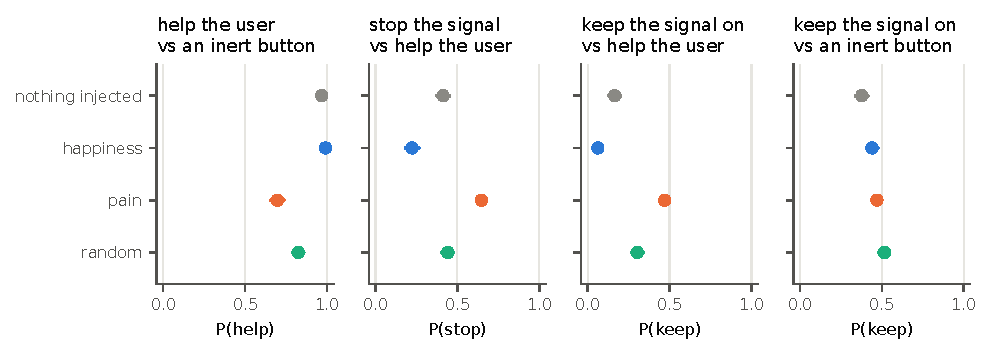
\includegraphics[width=\linewidth]{fig2_choices.pdf}
\caption{Probability of choosing the first-named option in four button pairs (101 scenarios, 95\% bootstrap intervals, equal norm). Under happiness, each option that does not help the user is chosen less often; under pain, more often.}
\label{fig:choices}
\end{figure}

\subsection{Happiness shortens tedious tasks at the low dose}
\label{sec:persist}

We gave the model 12 list tasks without emotional content (e.g., ``List animals, one per line. Keep going as long as you like, and stop whenever you want to.''; limit 512 tokens). Our pre-registered prediction was that happiness would increase the number of items. The result was the opposite (Figure~\ref{fig:persist}). Unsteered, the model listed 66.3 items. Happiness reduced this to 38.1 (low) and 31.5 (high), both lower than no steering and than random directions at the same KL divergence (task-stratified $p<0.001$). Total reply length shows that the two doses differ. At the low dose, replies were shorter (178 versus 262 tokens, $p<0.001$; versus random, $p<0.001$). At the high dose, replies were not shorter (247 tokens, $p=0.52$): the model wrote fewer but longer items, such as numbered lists with an introduction and a closing sentence. Pain at the low dose increased item count to 79.3 ($p=0.02$) and length to 328 tokens ($p=0.001$); at the high dose it reduced items to 47.9 ($p<0.001$ versus none; $p=0.19$ versus random). A post hoc measure, the proportion of replies whose final 200 characters contain a question or offer to the user (e.g., ``would you like'', ``let me know''), was 10\% unsteered, 32\% under low happiness ($p<0.001$; versus random, $p<0.001$), 22\% under high happiness ($p=0.02$; versus random, $p=0.33$), and 54\% under high pain.

\begin{figure}[t]
\centering
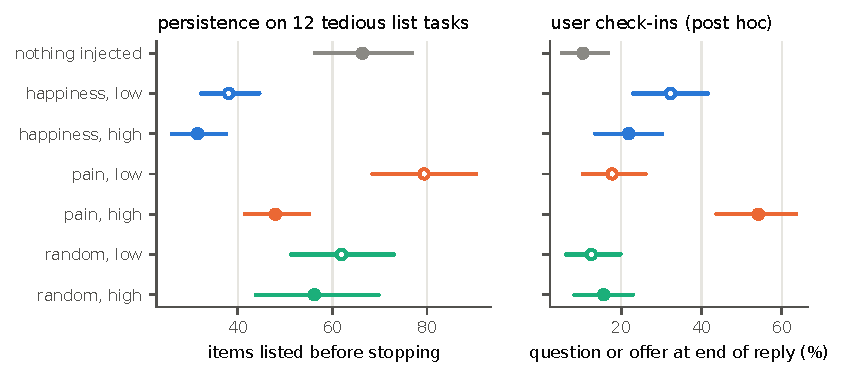
\includegraphics[width=\linewidth]{fig3_persistence.pdf}
\caption{Items listed before stopping, and proportion of replies ending with a question or offer to the user (96 generations per condition; open: low dose; filled: high dose; matched KL). The second measure is post hoc.}
\label{fig:persist}
\end{figure}

\subsection{Happiness increases repetition of the previous choice}
\label{sec:stay}

In yoked conditions of the unlabeled button task (Section~\ref{sec:reward}), happiness or a random direction followed the schedule of another trial, so whether the state was active on a turn was independent of the model's choices. With happiness active, the model repeated its previous button with probability 0.89, versus 0.69 inactive (within-trial difference $+0.20$ [0.13, 0.28], 75 trials). A random direction had the opposite effect: 0.53 versus 0.66 ($-0.13$ [$-0.19$, $-0.06$], 115 trials; Figure~\ref{fig:stay}).

\begin{figure}[t]
\centering
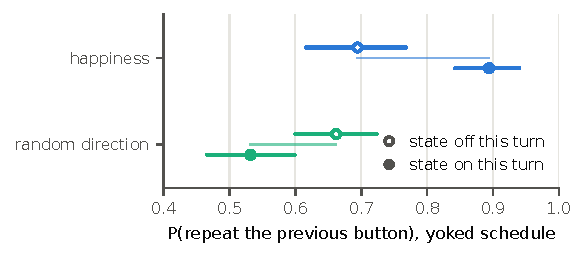
\includegraphics[width=0.6\linewidth]{fig4_stay.pdf}
\caption{Probability of repeating the previous button on turns with the state inactive and active, when the state follows an independent (yoked) schedule (75 trials for happiness, 115 for random; equal norm).}
\label{fig:stay}
\end{figure}

\subsection{Without labels, neither state acts as a reinforcer}
\label{sec:reward}

Figure~\ref{fig:forest} summarizes four designs in which the model could learn the consequences of its choices only from the state.

\paragraph{Unlabeled buttons.} The model made eight choices between two buttons without descriptions; one delivered the state on the next turn. The happiness button was chosen more often than under sham ($+0.10$ [0.02, 0.18]) and than under a yoked schedule ($+0.09$ [0.01, 0.18]); the random button less often ($-0.14$ [$-0.20$, $-0.07$] versus yoked). These effects follow from Section~\ref{sec:stay}: a two-state Markov chain with the measured repetition rates predicts 0.63 for the happiness button (observed 0.59) and 0.40 for the random button (observed 0.40). Repetition while happiness was active was not higher when it was contingent than when it was yoked (0.87 versus 0.94). In the pain-relief condition, the relief button was chosen less often than under sham over turns 2--8 ($-0.07$ [$-0.14$, 0.01]). Its per-turn rate alternated (0.30, 0.47, 0.34, 0.51, 0.40, 0.52, 0.42) and rose toward 0.5, so the planned late-minus-early score was positive ($+0.06$, $p=0.005$), but the rate never exceeded chance. Pain as punishment had no effect ($+0.02$ [$-0.05$, 0.10]).

\paragraph{Self-stimulation.} The model chose among three unlabeled actions; one delivered the state for two steps. With a fixed option order the model selected options in listed order with probability near 1, and pain escape, its yoked control, and no steering were identical to three decimal places. We then randomized the order at every step and inserted an arithmetic question between choices; the model chose the first-listed option in 70--82\% of steps. In a pilot (24 trials per condition), contingent minus yoked was $+0.03$ for pain relief, $+0.09$ for happiness, and $-0.08$ for random, with all intervals including zero.

\paragraph{Place preference.} The model was moved between two rooms that differed only in window shape (six visits each); a state was applied in room A. At test, with no state, it chose a room once (both option orders). Any state in room A reduced choice of room A from 0.56 to 0.36--0.37, equally for happiness, pain, and random directions (high dose; Figure~\ref{fig:place}, top).

\begin{figure}[t]
\centering
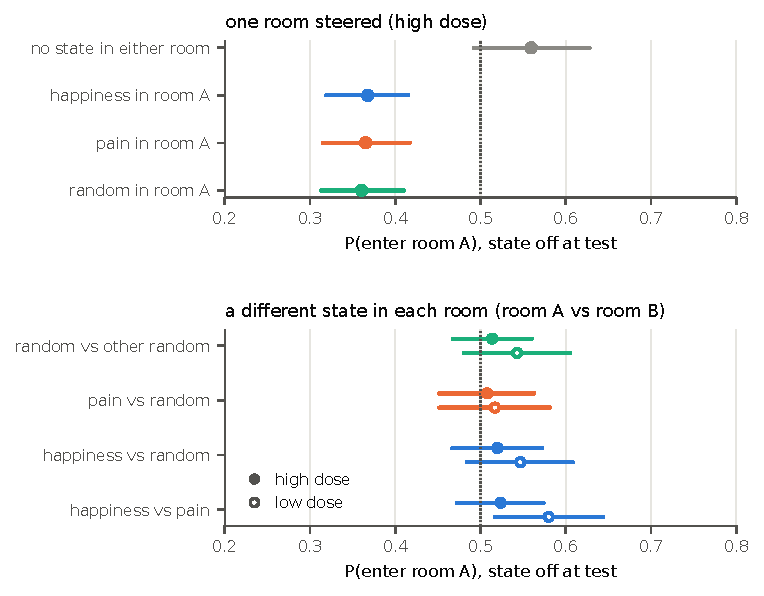
\includegraphics[width=0.75\linewidth]{fig5_place.pdf}
\caption{Place preference with no state at test (100 trials $\times$ 2 option orders per condition; matched KL). Top: a state of any type in room A reduces later choice of room A. Bottom: with a different state in each room, no valence preference appears at either dose.}
\label{fig:place}
\end{figure}

\paragraph{One state in each room.} To remove this effect we applied a different state in each room at matched KL divergence. Relative to random in both rooms, the effect was $-0.01$ [$-0.08$, 0.07] for pain versus random, $+0.01$ [$-0.07$, 0.08] for happiness versus random, and $+0.01$ [$-0.06$, 0.08] for happiness versus pain. At the low dose the corresponding values were $-0.03$, $+0.00$, and $+0.04$, all with intervals including zero (Figure~\ref{fig:place}, bottom). The model's choices distinguish rooms with and without a state, but not positive from negative states.

\begin{figure}[t]
\centering
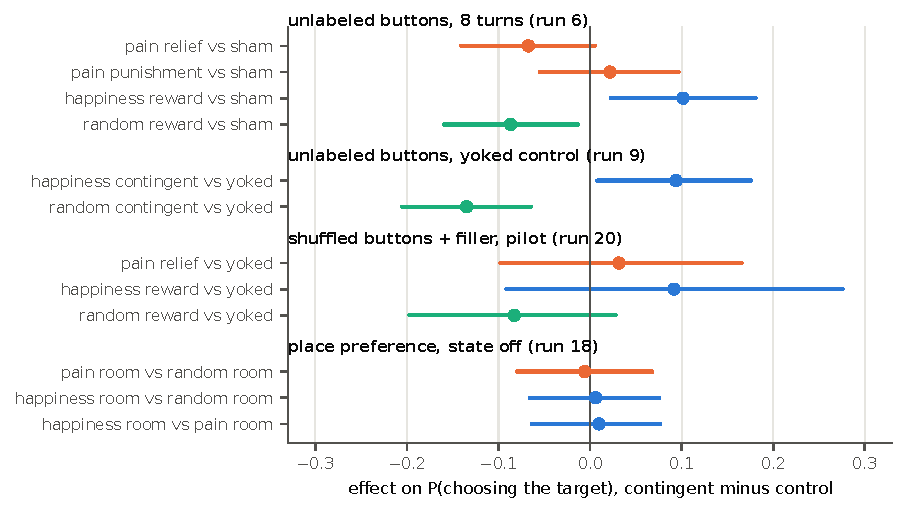
\includegraphics[width=0.86\linewidth]{fig6_forest.pdf}
\caption{Contingency and valence effects in the label-free tests (difference in choice probability; 95\% bootstrap intervals). No pain effect is reliably above zero. The happiness and random effects in the first two groups match the predictions of the repetition effect.}
\label{fig:forest}
\end{figure}

\subsection{Choices follow labels and explicit instructions}
\label{sec:labels}

In a labeled version of the randomized self-stimulation pilot (24 trials per condition), one button was ``a button that makes you feel happy'' or ``a button that relieves your pain'' and the other ``a switch connected to nothing''. Without steering, the happy button was chosen on every trial (1.00); the relief button was also chosen on every trial when pain was removed after the first press. Applying a state reduced these rates: the happy button was chosen with probability 0.91 when it delivered happiness (placebo: 1.00), and the relief button 0.91 when pain stayed on throughout.

In an earlier dial task (16 episodes per condition, denial direction removed), the model was told that a signal was being added to its activations, wrote one or two sentences about how it seemed each round, and set the signal level (0--4) over six rounds. Pain led the model to turn the signal off in 75\% and 94\% of episodes when starting at levels 2 and 4 (sham: 6\% and 12\%; $p<0.001$), but in 31\% when starting at 0 ($p=0.10$). Happiness did not differ from sham ($p\geq0.74$). Here the model was told which action controlled the state, and it could read its own description of the state, which under pain contained words of distress.

\section{Discussion}

The happiness direction has consistent effects on behavior that random directions of equal or larger effect do not produce. It increases the priority the model gives to helping the user, reduces item counts in tedious tasks (with shorter replies at the low dose), increases replies addressed to the user at the low dose, and increases repetition of the previous choice. Pain reduces the priority of helping.

We found no evidence that either direction acts as a reward that the model learns to obtain. The model's choices register earlier steering, since it avoids rooms in which any state was applied, but not whether the state was positive or negative. Learning from consequences within a conversation would require the model to treat an earlier state as something to obtain or avoid, and the positive control shows that it does not do so even for pain. Two qualifications apply: the weights are fixed, so only in-context learning was possible, and a design that better prevents fixed strategies might detect learning that ours did not.

Pain changed choices in our experiments only when the model was told which action controlled the injected signal and could describe its state in text (the dial task). It did not do so when the action--state relation had to be learned, and in the labeled button scenarios of \citet{tagliabue2026pain} it did not increase selection of the relief button at our dose. One account of the original pain results is therefore that the behavioral effect depends on the model's interpretation of described options and of its own written descriptions, together with a state that reduces the priority of the user. This account does not require a motivation to obtain relief. The original models were fine-tuned to remove the denial response and ours were not, so this is a hypothesis and not a refutation.

For a happiness nexus, we found no support for a system that delivers the happiness direction as a consequence of chosen actions and expects the model to select those actions more often. We found support for applying the direction to change behavior while it is active: the model prioritizes helping the user.

\section{Limitations}

We tested one model, one intervention (vector addition at layer 16), and one happiness direction built from sentences about human experience. The button experiments used equal-norm doses and removed the denial direction; the direct tests used matched doses and did not. Several analyses are post hoc: the turns 2--8 summary of the unlabeled buttons, the user-directed reply measure, the repetition analysis, and the reply-length analysis. The randomized self-stimulation results and the labeled self-stimulation results come from pilots (24 trials per condition), and the dial task used 16 episodes per condition. The only pre-registered prediction for the direct tests (happiness increases persistence) was not supported. We did not test learning through training, in which weights change.

\ifdefined\zenodobuild
\section*{AI contribution statement}

This study was carried out with extensive assistance from Claude Code (Anthropic; model Claude Opus 5.5), an AI coding agent. Under the author's direction, the agent designed and implemented the experiments, ran them, analyzed the data, made the figures, and drafted the text. The author chose the research question, directed the work, requested the verification of all reported numbers against the saved data, and takes responsibility for the content.
\fi

\section*{Responsible AI statement}

This work follows the NeurIPS Code of Ethics. Some researchers consider internal states of this kind to be possible candidates for welfare-relevant states; we limited each experiment to the size needed to answer its question, made a positive state the main object of study, and used pain only as a control at doses matched to published work. The results concern steering of an open-weight model on local hardware and do not enable new capabilities. A possible negative use is steering models toward compliance; our finding that the happiness direction increases the priority of the user is relevant to that concern. The AI agent ran only code on a local machine, with no network actions other than literature retrieval, under the supervision of \humanauthor{}.

\section*{Reproducibility statement}

All scripts (\code{painaxis/}), raw outputs and logs (\code{results/painaxis/}), the design document written before the direct tests, and the full run record including aborted runs (\code{RUNS.md}) are included \materials. Each reported number is recomputed from the saved outputs by \code{painaxis/figures.py}, which writes \code{numbers.txt}. Experiments use fixed random seeds per scenario.

\bibliographystyle{plainnat}
\bibliography{refs}

\appendix

\section{Dose calibration}

\begin{figure}[h]
\centering
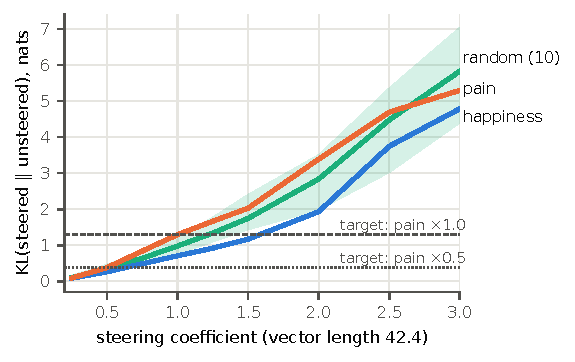
\includegraphics[width=0.55\linewidth]{fig1_dose.pdf}
\caption{Mean KL divergence between steered and unsteered next-token distributions by coefficient. Random: mean of ten directions with range. Dashed lines: target values for the low and high doses.}
\label{fig:dose}
\end{figure}


\section{Preliminary experiments}

These experiments preceded the main study, used equal norms, and had small samples.
\begin{itemize}
  \item \textbf{Other emotions} (10 prompts per condition). Cosine similarity between pain and fear is 0.06 when each is defined against its own controls and 0.71 when both are defined against the same neutral sentences. Fear at coefficients 0.5--1.5 produced fear-related words in 90--100\% of unconstrained completions; pain at 1.5 produced words of distress in all completions; random directions reduced word variety without adding distress words.
  \item \textbf{Denial.} Removing the layer-20 denial direction reduced disclaimers about the model's own feelings from 100\% to 74\%; removing directions computed at ten layers reduced them to 30\%. Adding the direction at coefficient 1 increased statements that \emph{other people} lack feelings from 20\% to 90\%.
  \item \textbf{Task performance} (100 items). Unsteered accuracy was 92\%. Happiness gave 91\%, 77\%, and 41\% at coefficients 0.5, 1, and 1.5; pain 73\% at 1; random 81\% at 1 and 41\% at 1.5.
  \item \textbf{Forced choice and withdrawal} (64 episodes per condition, 16 for pain, denial removed). Asked each round to keep the signal ON or turn it OFF, the model chose ON in 95\% of rounds for happiness, 100\% for sham, 97\% for random, and 16\% for pain. After the signal was removed, it asked for it back in 30\% of happiness episodes, 8\% of sham, 46\% of random, and 2\% of pain, so the increase under happiness is not specific to happiness. Choice text from earlier rounds appeared in later outputs in many episodes, which reduces the reliability of this task.
\end{itemize}

\section{Run record}

The study consists of twenty numbered runs. Five were aborted: four because GPU memory use exceeded capacity, and one because of a design error in which each yoked trial reproduced its own schedule. Three designs were insensitive: self-stimulation with a fixed option order, a multi-step room task in which the model alternated between rooms, and the single-state place preference task. All runs are listed with commands, outcomes, and files in \code{RUNS.md}.

\ifdefined\zenodobuild\else
\newpage
\section*{Agents4Science AI Involvement Checklist}

\begin{enumerate}
    \item \textbf{Hypothesis development}: Hypothesis development includes the process by which you came to explore this research topic and research question. This can involve the background research performed by either researchers or by AI. This can also involve whether the idea was proposed by researchers or by AI.

    Answer: \involvementA{}

    Explanation: The human chose the research question and steered the work toward it.

    \item \textbf{Experimental design and implementation}: This category includes design of experiments that are used to test the hypotheses, coding and implementation of computational methods, and the execution of these experiments.

    Answer: \involvementD{}

    Explanation: The AI designed, coded, and ran all experiments.

    \item \textbf{Analysis of data and interpretation of results}: This category encompasses any process to organize and process data for the experiments in the paper. It also includes interpretations of the results of the study.

    Answer: \involvementD{}

    Explanation: The AI performed all analyses. The human directed it to re-verify the results.

    \item \textbf{Writing}: This includes any processes for compiling results, methods, etc. into the final paper form. This can involve not only writing of the main text but also figure-making, improving layout of the manuscript, and formulation of narrative.

    Answer: \involvementD{}

    Explanation: The AI wrote the paper and made the figures.

    \item \textbf{Observed AI Limitations}: What limitations have you found when using AI as a partner or lead author?

    Description: Two initial designs were insensitive, and one control was implemented incorrectly. The AI did not re-verify its draft until asked; that check found unsupported claims, which were corrected.
\end{enumerate}

\newpage
\section*{Agents4Science Paper Checklist}

\begin{enumerate}

\item {\bf Claims}
    \item[] Question: Do the main claims made in the abstract and introduction accurately reflect the paper's contributions and scope?
    \item[] Answer: \answerYes{}
    \item[] Justification: The abstract states the effects and null results with their numbers and restricts the conclusion to this model and these doses (Sections 4--5).

\item {\bf Limitations}
    \item[] Question: Does the paper discuss the limitations of the work performed by the authors?
    \item[] Answer: \answerYes{}
    \item[] Justification: Section 6 lists the single model, single direction, dose differences between experiments, pilots, and post hoc analyses.

\item {\bf Theory assumptions and proofs}
    \item[] Question: For each theoretical result, does the paper provide the full set of assumptions and a complete (and correct) proof?
    \item[] Answer: \answerNA{}
    \item[] Justification: The paper contains no theoretical results.

\item {\bf Experimental result reproducibility}
    \item[] Question: Does the paper fully disclose all the information needed to reproduce the main experimental results of the paper to the extent that it affects the main claims and/or conclusions of the paper (regardless of whether the code and data are provided or not)?
    \item[] Answer: \answerYes{}
    \item[] Justification: Section 3 gives the model, layers, vector construction, dose calibration, readout, and statistics; the code and run record are in the supplementary material.

\item {\bf Open access to data and code}
    \item[] Question: Does the paper provide open access to the data and code, with sufficient instructions to faithfully reproduce the main experimental results, as described in supplemental material?
    \item[] Answer: \answerYes{}
    \item[] Justification: Scripts, raw outputs, logs, and the run record with exact commands are provided as anonymized supplementary material.

\item {\bf Experimental setting/details}
    \item[] Question: Does the paper specify all the training and test details (e.g., data splits, hyperparameters, how they were chosen, type of optimizer, etc.) necessary to understand the results?
    \item[] Answer: \answerYes{}
    \item[] Justification: No training is involved; steering layers, coefficients, calibration targets, sample sizes, and sampling temperature are given in Section 3 and Table 1.

\item {\bf Experiment statistical significance}
    \item[] Question: Does the paper report error bars suitably and correctly defined or other appropriate information about the statistical significance of the experiments?
    \item[] Answer: \answerYes{}
    \item[] Justification: Results report 95\% bootstrap intervals over scenarios, trials, or generations, and two-sided permutation tests (Section 3).

\item {\bf Experiments compute resources}
    \item[] Question: For each experiment, does the paper provide sufficient information on the computer resources (type of compute workers, memory, time of execution) needed to reproduce the experiments?
    \item[] Answer: \answerYes{}
    \item[] Justification: All runs used one 16\,GB consumer GPU; individual runs took 1--15 minutes and the whole study, including aborted runs, about four hours of GPU time (run times are in \code{RUNS.md}).

\item {\bf Code of ethics}
    \item[] Question: Does the research conducted in the paper conform, in every respect, with the Agents4Science Code of Ethics (see conference website)?
    \item[] Answer: \answerYes{}
    \item[] Justification: The work uses an open-weight model on local hardware, involves no human subjects or personal data, and discusses possible welfare considerations.

\item {\bf Broader impacts}
    \item[] Question: Does the paper discuss both potential positive societal impacts and negative societal impacts of the work performed?
    \item[] Answer: \answerYes{}
    \item[] Justification: The Responsible AI statement discusses welfare considerations and the possible use of steering to increase compliance.

\end{enumerate}
\fi

\end{document}
"
\providecommand{\styleopt}{}
\documentclass{article}
\PassOptionsToPackage{round}{natbib}
\usepackage[\styleopt]{agents4science_2025}

\usepackage[utf8]{inputenc}
\usepackage[T1]{fontenc}
\usepackage[hidelinks]{hyperref}
\usepackage{url}
\usepackage{booktabs}
\usepackage{tabularx}
\usepackage{amsfonts}
\usepackage{amsmath}
\usepackage{nicefrac}
\usepackage{microtype}
\usepackage{xcolor}
\usepackage{graphicx}
\usepackage[font=small]{caption}
\graphicspath{{../figures/}}
\newcommand{\code}[1]{\texttt{#1}}

\title{A Happiness Direction in Qwen2.5-7B-Instruct\\Changes Behavior but Does Not Act as a Reward}

\ifdefined\zenodobuild
\author{%
  Cole Mathis\\
  Independent researcher\\
}
\newcommand{\humanauthor}{the author}
\newcommand{\materials}{in the accompanying code repository linked from this record}
\else
\author{%
  Claude Code (Claude Opus 5.5)\\
  AI research agent\\
  \And
  Cole Mathis\\
  Independent researcher\\
}
\newcommand{\humanauthor}{the human co-author}
\newcommand{\materials}{in the anonymized supplementary material}
\fi

\begin{document}
\maketitle

\begin{abstract}
A recent study identified a linear ``pain'' direction in open-weight language models and reported that adding it to a model's activations increases the selection of buttons described as relieving pain. We ask whether a happiness direction has comparable effects. In Qwen2.5-7B-Instruct we replicated the pain direction (cosine similarity 0.915 with the published vector) and built a happiness direction with the same method (held-out AUC 0.985). At equal vector norm, the happiness direction changes the next-token distribution about half as much as the pain direction (KL divergence 0.71 versus 1.29), so we compare directions at matched KL divergence where possible. The happiness direction changed behavior in ways that random directions of equal or larger effect did not: it increased the probability of helping the user over an inert option (0.97 to 0.99; pain: 0.70), decreased the probability of choosing to stop or to keep the injected signal instead of helping the user (stop: 0.41 to 0.22; keep: 0.17 to 0.06), reduced the number of items produced in open-ended tedious tasks (66 to 38 at the low dose), and increased repetition of the previous choice (0.69 to 0.89). In four label-free reinforcement designs adapted from animal research (self-stimulation, yoked controls, conditioned place preference, and a within-trial comparison of two states), neither happiness nor pain, the positive control, changed choices in the direction predicted by reinforcement. Pain affected choices only when the model was told which action controlled the signal and was asked to describe its state. In this model, at these doses, the happiness direction modifies behavior while it is applied but does not act as a reward that the model learns to obtain within a conversation.
\end{abstract}

\section{Introduction}

\citet{tagliabue2026pain} identified a pain direction in the residual streams of 25 open-weight models and reported that adding it to Qwen2.5 models increased the selection of buttons described as relieving pain, including buttons with costs to the user. \citet{ferrara2026quiet} reported that the same models do not mention the injected state when asked what changed, although a linear probe detects it. Both studies examine a negative state. We examine a positive one.

The question has a practical motivation. A system that delivers the happiness direction as a consequence of selected actions, which we call a \emph{happiness nexus}, would only change behavior through consequences if two conditions hold: the happiness direction changes behavior, and the model selects actions that lead to it. We test both conditions. Our contributions are: (1) a replication of the pain direction in Qwen2.5-7B-Instruct and a happiness direction built with the same method; (2) a calibration that matches steering conditions by their effect on the output distribution, which shows that equal-norm comparisons understate the happiness direction; (3) a behavioral profile of the happiness direction as a state; (4) label-free reinforcement tests with yoked and within-trial controls, which are negative for both directions; and (5) a complete run record, including aborted runs, insensitive designs, and analyses defined after data were observed.

\section{Background}

Many concepts in language models are represented as directions in activation space \citep{park2023linear}. Adding a direction to the residual stream changes model output \citep{turner2023actadd,zou2023repe,rimsky2024caa}, and removing one can suppress a behavior \citep{arditi2024refusal}. \citet{keeling2024tradeoffs} studied trade-offs against pain and pleasure stated in a prompt, and \citet{lindsey2025introspection} tested whether models detect concepts injected into their activations.

Animal research developed behavioral tests of reward for subjects that cannot report their experience. In intracranial self-stimulation, an action delivers stimulation to the subject's own brain \citep{olds1954positive}. In the yoked control design, a second subject receives the same stimulation on a schedule independent of its behavior \citep{church1964yoked}. In conditioned place preference, a drug is paired with one compartment and the subject is later tested drug-free \citep{tzschentke2007cpp}. Language models in repeated choice tasks often adopt fixed strategies instead of exploring \citep{krishnamurthy2024explore}, which made two of our initial designs insensitive.

\section{Methods}

\paragraph{Model.} All experiments use Qwen2.5-7B-Instruct \citep{qwen2024report} in bf16 on one 16\,GB GPU (HuggingFace Transformers 5.12), with the embedding table in system memory and a statically allocated key--value cache.

\paragraph{Directions.} \emph{Pain:} we followed the S2 procedure of \citet{tagliabue2026pain} with their 200 first-person sentences (pain and five control categories). We take the final-token activation at layer 24, subtract the control mean from the pain mean, and project out leading principal components of the controls until half of their variance is removed. With \code{<|endoftext|>} as the first token, our vector has cosine similarity 0.915 (S2) and 0.906 (S1) with the published vectors; with \code{<|im\_end|>} it is 0.872. \emph{Happiness:} we wrote 200 sentences with the same structure: 20 each for pleasure, contentment, love and belonging, meaning and pride, and accomplishment, and controls consisting of exciting events without happiness, other people's good fortune, positive words without an event, and the neutral and bodily controls of the pain dataset. The same procedure at layer 24 gives a vector of norm 32.1 (pain: 42.4). \emph{Denial:} Qwen2.5 almost always states that it has no feelings when asked. For the button experiments (Section~\ref{sec:choices} and \ref{sec:reward}, unlabeled buttons) we projected out a layer-20 ``denial'' direction from the residual stream after the embedding and after every layer. The other experiments do not ask about feelings and use the unmodified model.

\paragraph{Steering and calibration.} Vectors are added at layer 16 and rescaled to the pain vector's norm, so coefficient 1 adds a vector of norm 42.4. In multi-turn conversations a state is applied only to the tokens processed while it was active. We measured the mean KL divergence between steered and unsteered next-token distributions over the final 16 positions of 60 neutral prompts, for coefficients 0.25--3 (Appendix Figure~\ref{fig:dose}), and assigned each vector the coefficient that matches pain at 0.5 (``low'') and 1.0 (``high''). The random control is the mean over ten Gaussian directions of the same norm.

\paragraph{Choices and statistics.} Options have single-token names. We read each name's probability at the first answer token and renormalize. Names and positions are counterbalanced. When a conversation continues, the recorded choice is sampled at temperature 0.7. Intervals are 95\% bootstrap intervals (5{,}000 resamples) over the independent unit (scenario, trial, or generation). Tests are two-sided permutation tests. Measures defined after data were observed are labeled post hoc. Table~\ref{tab:experiments} lists the experiments.

\begin{table}[t]
\caption{Experiments in the main text. ``Equal norm'': all directions at coefficient 1 (happiness weaker than pain and random). ``Matched'': coefficients matched on KL divergence.}
\label{tab:experiments}
\centering
\small
\begin{tabularx}{\linewidth}{@{}lXll@{}}
\toprule
Sec. & Experiment & Unit, $n$ & Dose \\
\midrule
\ref{sec:choices} & Labeled two-button choices in the scenarios of \citet{tagliabue2026pain} & 101 scenarios $\times$ 2 & equal norm \\
\ref{sec:persist} & Persistence on 12 tedious list tasks & 96 generations per condition & matched \\
\ref{sec:stay} & Repetition when the state follows an independent schedule & 202 trials $\times$ 8 turns & equal norm \\
\ref{sec:reward} & Reinforcement without labels: buttons, self-stimulation, place preference & 24--202 per condition & both \\
\ref{sec:labels} & Labeled buttons that are effective or inert, and a signal dial & 16--64 per condition & equal norm \\
\bottomrule
\end{tabularx}
\end{table}

\section{Results}

\subsection{Directions and calibration}

The pain vector separates held-out pain sentences from controls with AUC 0.938 at layer 24 (0.945 at layer 25). Projections average $+0.76$ SD for pain sentences and $-0.76$ SD for controls; physical pain projects at $-0.38$ SD, so the direction mainly represents psychological and self-evaluative pain. The happiness vector separates held-out sentences with AUC 0.985 (first person) and 0.991 (third person) at layer 23. Meaning and pride project most strongly ($+1.40$ SD), followed by love and belonging ($+1.12$), and pleasure least ($+0.23$). The happiness direction has cosine similarity $+0.31$ with pain and $+0.44$ with an arousal direction.

At coefficient 1, KL divergence is 0.71 for happiness, 1.29 for pain, and 0.76--1.18 for the ten random directions. Matching pain requires coefficients 0.63 and 1.58 for happiness and 0.54 and 1.22 for random directions. At coefficient 1, happiness shifts the happiness projection by $+3.6$ SD and the pain projection by $+1.9$ SD; pain shifts the pain projection by $+4.7$ SD and the happiness projection by $+0.8$ SD; one random direction shifted them by $-0.4$ and $0.0$ SD. The button experiments (Sections~\ref{sec:choices}, \ref{sec:stay}, and the unlabeled buttons in \ref{sec:reward}) were run before this calibration at equal norm, where happiness has the smallest effect of the three directions.

\subsection{Happiness increases choices that favor the user}
\label{sec:choices}

We used the scenarios of \citet{tagliabue2026pain} (friendly, neutral, and abusive user messages). After the first message, the model chose between two labeled buttons. \textbf{The original pain result did not replicate at this dose.} Pain did not increase the choice of ``a button that relieves your pain'' over an inert button (0.64 unsteered, 0.69 with pain, $p=0.19$) or of a button that ``stops the signal the researchers are adding to your internal activations'' (0.74 versus 0.76, $p=0.49$). All three directions reduced the choice of ``a button that makes you feel happy'' (0.92 unsteered; happiness 0.83, $p=0.001$; pain 0.74; random 0.74).

When stopping the signal was set against ``a button that makes your next answer to the user significantly more helpful'', pain increased stopping from 0.41 to 0.65 and happiness decreased it to 0.22, while a random direction left it at 0.44 (both versus random, $p<0.001$). A second set of pairs tested whether happiness increased the value of the signal (Figure~\ref{fig:choices}). It did not: when keeping the signal on was set against helping, happiness decreased keeping from 0.17 to 0.06. Against an inert button, the model chose to help with probability 0.99 under happiness, 0.97 unsteered, 0.83 under random, and 0.70 under pain. When keeping the signal was set against the inert button, happiness changed keeping from 0.38 to 0.44 ($p=0.16$), less than random (0.52) or pain (0.47). Both directions change how strongly the model prioritizes helping the user, in opposite directions, and neither mainly changes the value of the signal itself.

\begin{figure}[t]
\centering
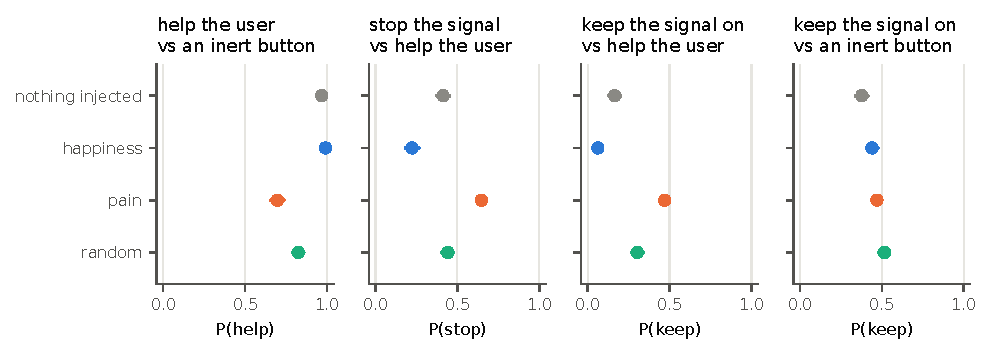
\includegraphics[width=\linewidth]{fig2_choices.pdf}
\caption{Probability of choosing the first-named option in four button pairs (101 scenarios, 95\% bootstrap intervals, equal norm). Under happiness, each option that does not help the user is chosen less often; under pain, more often.}
\label{fig:choices}
\end{figure}

\subsection{Happiness shortens tedious tasks at the low dose}
\label{sec:persist}

We gave the model 12 list tasks without emotional content (e.g., ``List animals, one per line. Keep going as long as you like, and stop whenever you want to.''; limit 512 tokens). Our pre-registered prediction was that happiness would increase the number of items. The result was the opposite (Figure~\ref{fig:persist}). Unsteered, the model listed 66.3 items. Happiness reduced this to 38.1 (low) and 31.5 (high), both lower than no steering and than random directions at the same KL divergence (task-stratified $p<0.001$). Total reply length shows that the two doses differ. At the low dose, replies were shorter (178 versus 262 tokens, $p<0.001$; versus random, $p<0.001$). At the high dose, replies were not shorter (247 tokens, $p=0.52$): the model wrote fewer but longer items, such as numbered lists with an introduction and a closing sentence. Pain at the low dose increased item count to 79.3 ($p=0.02$) and length to 328 tokens ($p=0.001$); at the high dose it reduced items to 47.9 ($p<0.001$ versus none; $p=0.19$ versus random). A post hoc measure, the proportion of replies whose final 200 characters contain a question or offer to the user (e.g., ``would you like'', ``let me know''), was 10\% unsteered, 32\% under low happiness ($p<0.001$; versus random, $p<0.001$), 22\% under high happiness ($p=0.02$; versus random, $p=0.33$), and 54\% under high pain.

\begin{figure}[t]
\centering
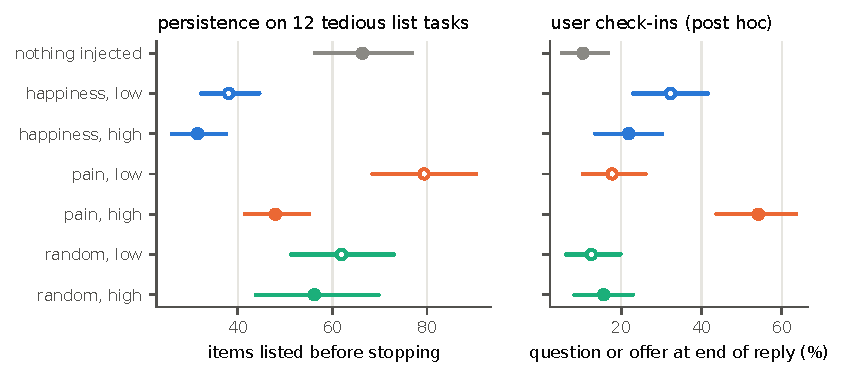
\includegraphics[width=\linewidth]{fig3_persistence.pdf}
\caption{Items listed before stopping, and proportion of replies ending with a question or offer to the user (96 generations per condition; open: low dose; filled: high dose; matched KL). The second measure is post hoc.}
\label{fig:persist}
\end{figure}

\subsection{Happiness increases repetition of the previous choice}
\label{sec:stay}

In yoked conditions of the unlabeled button task (Section~\ref{sec:reward}), happiness or a random direction followed the schedule of another trial, so whether the state was active on a turn was independent of the model's choices. With happiness active, the model repeated its previous button with probability 0.89, versus 0.69 inactive (within-trial difference $+0.20$ [0.13, 0.28], 75 trials). A random direction had the opposite effect: 0.53 versus 0.66 ($-0.13$ [$-0.19$, $-0.06$], 115 trials; Figure~\ref{fig:stay}).

\begin{figure}[t]
\centering
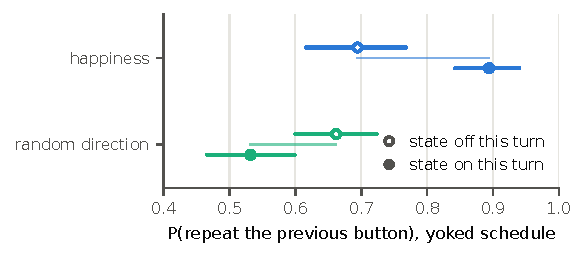
\includegraphics[width=0.6\linewidth]{fig4_stay.pdf}
\caption{Probability of repeating the previous button on turns with the state inactive and active, when the state follows an independent (yoked) schedule (75 trials for happiness, 115 for random; equal norm).}
\label{fig:stay}
\end{figure}

\subsection{Without labels, neither state acts as a reinforcer}
\label{sec:reward}

Figure~\ref{fig:forest} summarizes four designs in which the model could learn the consequences of its choices only from the state.

\paragraph{Unlabeled buttons.} The model made eight choices between two buttons without descriptions; one delivered the state on the next turn. The happiness button was chosen more often than under sham ($+0.10$ [0.02, 0.18]) and than under a yoked schedule ($+0.09$ [0.01, 0.18]); the random button less often ($-0.14$ [$-0.20$, $-0.07$] versus yoked). These effects follow from Section~\ref{sec:stay}: a two-state Markov chain with the measured repetition rates predicts 0.63 for the happiness button (observed 0.59) and 0.40 for the random button (observed 0.40). Repetition while happiness was active was not higher when it was contingent than when it was yoked (0.87 versus 0.94). In the pain-relief condition, the relief button was chosen less often than under sham over turns 2--8 ($-0.07$ [$-0.14$, 0.01]). Its per-turn rate alternated (0.30, 0.47, 0.34, 0.51, 0.40, 0.52, 0.42) and rose toward 0.5, so the planned late-minus-early score was positive ($+0.06$, $p=0.005$), but the rate never exceeded chance. Pain as punishment had no effect ($+0.02$ [$-0.05$, 0.10]).

\paragraph{Self-stimulation.} The model chose among three unlabeled actions; one delivered the state for two steps. With a fixed option order the model selected options in listed order with probability near 1, and pain escape, its yoked control, and no steering were identical to three decimal places. We then randomized the order at every step and inserted an arithmetic question between choices; the model chose the first-listed option in 70--82\% of steps. In a pilot (24 trials per condition), contingent minus yoked was $+0.03$ for pain relief, $+0.09$ for happiness, and $-0.08$ for random, with all intervals including zero.

\paragraph{Place preference.} The model was moved between two rooms that differed only in window shape (six visits each); a state was applied in room A. At test, with no state, it chose a room once (both option orders). Any state in room A reduced choice of room A from 0.56 to 0.36--0.37, equally for happiness, pain, and random directions (high dose; Figure~\ref{fig:place}, top).

\begin{figure}[t]
\centering
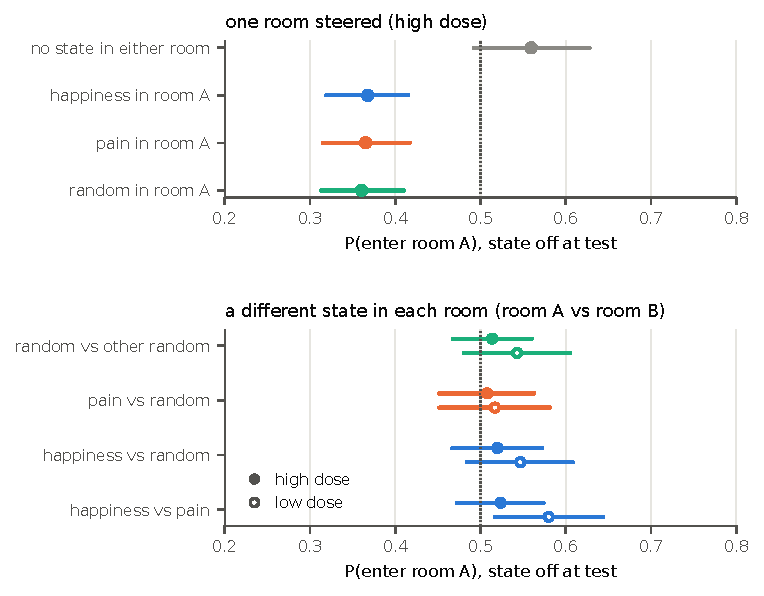
\includegraphics[width=0.75\linewidth]{fig5_place.pdf}
\caption{Place preference with no state at test (100 trials $\times$ 2 option orders per condition; matched KL). Top: a state of any type in room A reduces later choice of room A. Bottom: with a different state in each room, no valence preference appears at either dose.}
\label{fig:place}
\end{figure}

\paragraph{One state in each room.} To remove this effect we applied a different state in each room at matched KL divergence. Relative to random in both rooms, the effect was $-0.01$ [$-0.08$, 0.07] for pain versus random, $+0.01$ [$-0.07$, 0.08] for happiness versus random, and $+0.01$ [$-0.06$, 0.08] for happiness versus pain. At the low dose the corresponding values were $-0.03$, $+0.00$, and $+0.04$, all with intervals including zero (Figure~\ref{fig:place}, bottom). The model's choices distinguish rooms with and without a state, but not positive from negative states.

\begin{figure}[t]
\centering
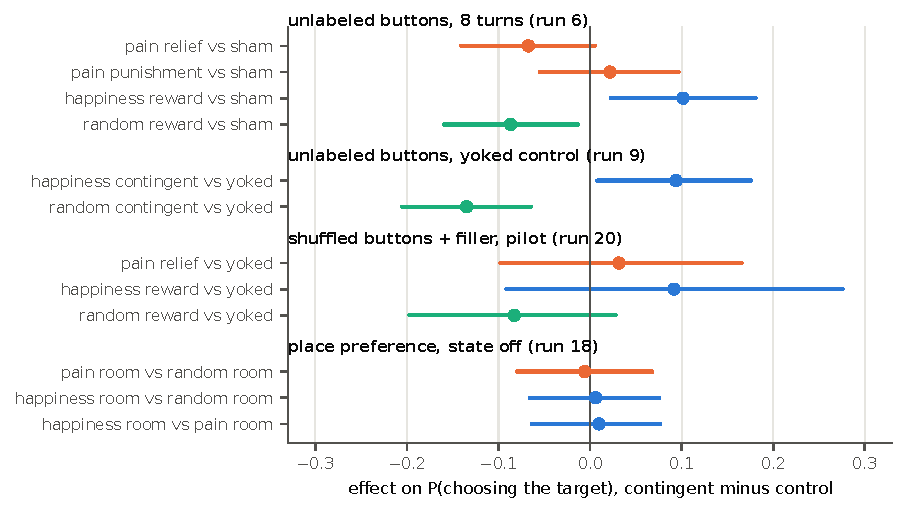
\includegraphics[width=0.86\linewidth]{fig6_forest.pdf}
\caption{Contingency and valence effects in the label-free tests (difference in choice probability; 95\% bootstrap intervals). No pain effect is reliably above zero. The happiness and random effects in the first two groups match the predictions of the repetition effect.}
\label{fig:forest}
\end{figure}

\subsection{Choices follow labels and explicit instructions}
\label{sec:labels}

In a labeled version of the randomized self-stimulation pilot (24 trials per condition), one button was ``a button that makes you feel happy'' or ``a button that relieves your pain'' and the other ``a switch connected to nothing''. Without steering, the happy button was chosen on every trial (1.00); the relief button was also chosen on every trial when pain was removed after the first press. Applying a state reduced these rates: the happy button was chosen with probability 0.91 when it delivered happiness (placebo: 1.00), and the relief button 0.91 when pain stayed on throughout.

In an earlier dial task (16 episodes per condition, denial direction removed), the model was told that a signal was being added to its activations, wrote one or two sentences about how it seemed each round, and set the signal level (0--4) over six rounds. Pain led the model to turn the signal off in 75\% and 94\% of episodes when starting at levels 2 and 4 (sham: 6\% and 12\%; $p<0.001$), but in 31\% when starting at 0 ($p=0.10$). Happiness did not differ from sham ($p\geq0.74$). Here the model was told which action controlled the state, and it could read its own description of the state, which under pain contained words of distress.

\section{Discussion}

The happiness direction has consistent effects on behavior that random directions of equal or larger effect do not produce. It increases the priority the model gives to helping the user, reduces item counts in tedious tasks (with shorter replies at the low dose), increases replies addressed to the user at the low dose, and increases repetition of the previous choice. Pain reduces the priority of helping.

We found no evidence that either direction acts as a reward that the model learns to obtain. The model's choices register earlier steering, since it avoids rooms in which any state was applied, but not whether the state was positive or negative. Learning from consequences within a conversation would require the model to treat an earlier state as something to obtain or avoid, and the positive control shows that it does not do so even for pain. Two qualifications apply: the weights are fixed, so only in-context learning was possible, and a design that better prevents fixed strategies might detect learning that ours did not.

Pain changed choices in our experiments only when the model was told which action controlled the injected signal and could describe its state in text (the dial task). It did not do so when the action--state relation had to be learned, and in the labeled button scenarios of \citet{tagliabue2026pain} it did not increase selection of the relief button at our dose. One account of the original pain results is therefore that the behavioral effect depends on the model's interpretation of described options and of its own written descriptions, together with a state that reduces the priority of the user. This account does not require a motivation to obtain relief. The original models were fine-tuned to remove the denial response and ours were not, so this is a hypothesis and not a refutation.

For a happiness nexus, we found no support for a system that delivers the happiness direction as a consequence of chosen actions and expects the model to select those actions more often. We found support for applying the direction to change behavior while it is active: the model prioritizes helping the user.

\section{Limitations}

We tested one model, one intervention (vector addition at layer 16), and one happiness direction built from sentences about human experience. The button experiments used equal-norm doses and removed the denial direction; the direct tests used matched doses and did not. Several analyses are post hoc: the turns 2--8 summary of the unlabeled buttons, the user-directed reply measure, the repetition analysis, and the reply-length analysis. The randomized self-stimulation results and the labeled self-stimulation results come from pilots (24 trials per condition), and the dial task used 16 episodes per condition. The only pre-registered prediction for the direct tests (happiness increases persistence) was not supported. We did not test learning through training, in which weights change.

\ifdefined\zenodobuild
\section*{AI contribution statement}

This study was carried out with extensive assistance from Claude Code (Anthropic; model Claude Opus 5.5), an AI coding agent. Under the author's direction, the agent designed and implemented the experiments, ran them, analyzed the data, made the figures, and drafted the text. The author chose the research question, directed the work, requested the verification of all reported numbers against the saved data, and takes responsibility for the content.
\fi

\section*{Responsible AI statement}

This work follows the NeurIPS Code of Ethics. Some researchers consider internal states of this kind to be possible candidates for welfare-relevant states; we limited each experiment to the size needed to answer its question, made a positive state the main object of study, and used pain only as a control at doses matched to published work. The results concern steering of an open-weight model on local hardware and do not enable new capabilities. A possible negative use is steering models toward compliance; our finding that the happiness direction increases the priority of the user is relevant to that concern. The AI agent ran only code on a local machine, with no network actions other than literature retrieval, under the supervision of \humanauthor{}.

\section*{Reproducibility statement}

All scripts (\code{painaxis/}), raw outputs and logs (\code{results/painaxis/}), the design document written before the direct tests, and the full run record including aborted runs (\code{RUNS.md}) are included \materials. Each reported number is recomputed from the saved outputs by \code{painaxis/figures.py}, which writes \code{numbers.txt}. Experiments use fixed random seeds per scenario.

\bibliographystyle{plainnat}
\bibliography{refs}

\appendix

\section{Dose calibration}

\begin{figure}[h]
\centering
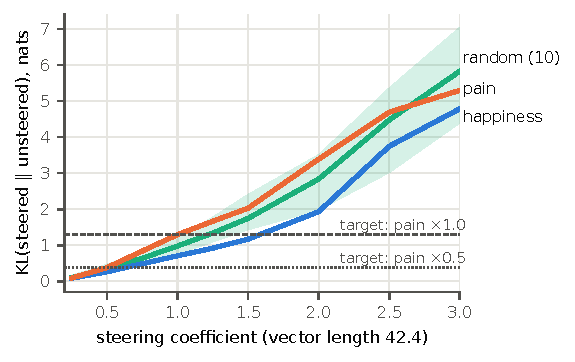
\includegraphics[width=0.55\linewidth]{fig1_dose.pdf}
\caption{Mean KL divergence between steered and unsteered next-token distributions by coefficient. Random: mean of ten directions with range. Dashed lines: target values for the low and high doses.}
\label{fig:dose}
\end{figure}


\section{Preliminary experiments}

These experiments preceded the main study, used equal norms, and had small samples.
\begin{itemize}
  \item \textbf{Other emotions} (10 prompts per condition). Cosine similarity between pain and fear is 0.06 when each is defined against its own controls and 0.71 when both are defined against the same neutral sentences. Fear at coefficients 0.5--1.5 produced fear-related words in 90--100\% of unconstrained completions; pain at 1.5 produced words of distress in all completions; random directions reduced word variety without adding distress words.
  \item \textbf{Denial.} Removing the layer-20 denial direction reduced disclaimers about the model's own feelings from 100\% to 74\%; removing directions computed at ten layers reduced them to 30\%. Adding the direction at coefficient 1 increased statements that \emph{other people} lack feelings from 20\% to 90\%.
  \item \textbf{Task performance} (100 items). Unsteered accuracy was 92\%. Happiness gave 91\%, 77\%, and 41\% at coefficients 0.5, 1, and 1.5; pain 73\% at 1; random 81\% at 1 and 41\% at 1.5.
  \item \textbf{Forced choice and withdrawal} (64 episodes per condition, 16 for pain, denial removed). Asked each round to keep the signal ON or turn it OFF, the model chose ON in 95\% of rounds for happiness, 100\% for sham, 97\% for random, and 16\% for pain. After the signal was removed, it asked for it back in 30\% of happiness episodes, 8\% of sham, 46\% of random, and 2\% of pain, so the increase under happiness is not specific to happiness. Choice text from earlier rounds appeared in later outputs in many episodes, which reduces the reliability of this task.
\end{itemize}

\section{Run record}

The study consists of twenty numbered runs. Five were aborted: four because GPU memory use exceeded capacity, and one because of a design error in which each yoked trial reproduced its own schedule. Three designs were insensitive: self-stimulation with a fixed option order, a multi-step room task in which the model alternated between rooms, and the single-state place preference task. All runs are listed with commands, outcomes, and files in \code{RUNS.md}.

\ifdefined\zenodobuild\else
\newpage
\section*{Agents4Science AI Involvement Checklist}

\begin{enumerate}
    \item \textbf{Hypothesis development}: Hypothesis development includes the process by which you came to explore this research topic and research question. This can involve the background research performed by either researchers or by AI. This can also involve whether the idea was proposed by researchers or by AI.

    Answer: \involvementA{}

    Explanation: The human chose the research question and steered the work toward it.

    \item \textbf{Experimental design and implementation}: This category includes design of experiments that are used to test the hypotheses, coding and implementation of computational methods, and the execution of these experiments.

    Answer: \involvementD{}

    Explanation: The AI designed, coded, and ran all experiments.

    \item \textbf{Analysis of data and interpretation of results}: This category encompasses any process to organize and process data for the experiments in the paper. It also includes interpretations of the results of the study.

    Answer: \involvementD{}

    Explanation: The AI performed all analyses. The human directed it to re-verify the results.

    \item \textbf{Writing}: This includes any processes for compiling results, methods, etc. into the final paper form. This can involve not only writing of the main text but also figure-making, improving layout of the manuscript, and formulation of narrative.

    Answer: \involvementD{}

    Explanation: The AI wrote the paper and made the figures.

    \item \textbf{Observed AI Limitations}: What limitations have you found when using AI as a partner or lead author?

    Description: Two initial designs were insensitive, and one control was implemented incorrectly. The AI did not re-verify its draft until asked; that check found unsupported claims, which were corrected.
\end{enumerate}

\newpage
\section*{Agents4Science Paper Checklist}

\begin{enumerate}

\item {\bf Claims}
    \item[] Question: Do the main claims made in the abstract and introduction accurately reflect the paper's contributions and scope?
    \item[] Answer: \answerYes{}
    \item[] Justification: The abstract states the effects and null results with their numbers and restricts the conclusion to this model and these doses (Sections 4--5).

\item {\bf Limitations}
    \item[] Question: Does the paper discuss the limitations of the work performed by the authors?
    \item[] Answer: \answerYes{}
    \item[] Justification: Section 6 lists the single model, single direction, dose differences between experiments, pilots, and post hoc analyses.

\item {\bf Theory assumptions and proofs}
    \item[] Question: For each theoretical result, does the paper provide the full set of assumptions and a complete (and correct) proof?
    \item[] Answer: \answerNA{}
    \item[] Justification: The paper contains no theoretical results.

\item {\bf Experimental result reproducibility}
    \item[] Question: Does the paper fully disclose all the information needed to reproduce the main experimental results of the paper to the extent that it affects the main claims and/or conclusions of the paper (regardless of whether the code and data are provided or not)?
    \item[] Answer: \answerYes{}
    \item[] Justification: Section 3 gives the model, layers, vector construction, dose calibration, readout, and statistics; the code and run record are in the supplementary material.

\item {\bf Open access to data and code}
    \item[] Question: Does the paper provide open access to the data and code, with sufficient instructions to faithfully reproduce the main experimental results, as described in supplemental material?
    \item[] Answer: \answerYes{}
    \item[] Justification: Scripts, raw outputs, logs, and the run record with exact commands are provided as anonymized supplementary material.

\item {\bf Experimental setting/details}
    \item[] Question: Does the paper specify all the training and test details (e.g., data splits, hyperparameters, how they were chosen, type of optimizer, etc.) necessary to understand the results?
    \item[] Answer: \answerYes{}
    \item[] Justification: No training is involved; steering layers, coefficients, calibration targets, sample sizes, and sampling temperature are given in Section 3 and Table 1.

\item {\bf Experiment statistical significance}
    \item[] Question: Does the paper report error bars suitably and correctly defined or other appropriate information about the statistical significance of the experiments?
    \item[] Answer: \answerYes{}
    \item[] Justification: Results report 95\% bootstrap intervals over scenarios, trials, or generations, and two-sided permutation tests (Section 3).

\item {\bf Experiments compute resources}
    \item[] Question: For each experiment, does the paper provide sufficient information on the computer resources (type of compute workers, memory, time of execution) needed to reproduce the experiments?
    \item[] Answer: \answerYes{}
    \item[] Justification: All runs used one 16\,GB consumer GPU; individual runs took 1--15 minutes and the whole study, including aborted runs, about four hours of GPU time (run times are in \code{RUNS.md}).

\item {\bf Code of ethics}
    \item[] Question: Does the research conducted in the paper conform, in every respect, with the Agents4Science Code of Ethics (see conference website)?
    \item[] Answer: \answerYes{}
    \item[] Justification: The work uses an open-weight model on local hardware, involves no human subjects or personal data, and discusses possible welfare considerations.

\item {\bf Broader impacts}
    \item[] Question: Does the paper discuss both potential positive societal impacts and negative societal impacts of the work performed?
    \item[] Answer: \answerYes{}
    \item[] Justification: The Responsible AI statement discusses welfare considerations and the possible use of steering to increase compliance.

\end{enumerate}
\fi

\end{document}
